% !TEX root = paper.tex

\section{Introduction}

%\textbf{{[A general history on HI]}}

The main emphasis of the ultra-relativistic heavy-ion collision programs at the Relativistic Heavy Ion Collider (RHIC) and the Large Hadron Collider (LHC) is to study the deconfined phase of strongly interacting nuclear matter, the Quark-Gluon Plasma (QGP). 
This matter exhibits strong collective and anisotropic flow in the plane transverse to the beam direction, which is driven by anisotropic pressure gradients, resulting in more particles emitted in the direction of the largest gradients.
The large elliptic flow discovered at RHIC energies~\cite{Ackermann:2000tr} is also observed at LHC energies~\cite{Aamodt:2010pa,Adam:2016izf}. This was predicted by calculations utilizing viscous hydrodynamics~\cite{Romatschke:2007mq,Shen:2011eg,Schenke:2011zz,Bozek:2012qs,Gale:2012rq,Hirano:2010je}.
%and microscopic transport models ~\cite{Xu:2007jv}.  
These calculations also demonstrated that the shear viscosity to the entropy density ratio ($\eta/s$) of the QGP in heavy-ion collisions at RHIC and LHC energies is close to a universal lower bound $1/4\pi$~\cite{Kovtun:2004de}.

The temperature dependence of $\eta/s$ has some generic features that most known fluids obey. For instance, one such general behavior is that this ratio typically reaches its minimum value close to the phase transition region~\cite{Lacey:2006bc}. 
It was shown, using kinetic theory and quantum mechanical considerations~\cite{PhysRevD.31.53}, that $\eta/s\sim0.1$ would be the correct order of magnitude for the lowest possible shear viscosity to entropy density ratio value found in nature. Later it was demonstrated that an exact lower bound $(\eta/s)_{\rm min}=1/4\pi\approx0.08$ can be calculated using AdS/CFT correspondence~\cite{Kovtun:2004de}. Hydrodynamical simulations also support the view that $\eta/s$ of the QGP is close to the lower bound~\cite{Gale:2012rq}.
%This may have important implications for other fundamental physics goals. 
It is argued that such a low value might imply that thermodynamic trajectories for the expanding matter would lie close to the quantum chromodynamics (QCD) critical end point, which is another subject of intensive experimental study~\cite{Lacey:2006bc,Csernai:2006zz}.
%which in turn would gain better prospects to search of critical end point~\cite{PhysRevLett.98.092301}.

%The magnitude of the anisotropic flow has been to found to be sensitive to the transport properties, as well as the space-momentum profile in the initial state~\cite{}. 
Anisotropic flow~\cite{Ollitrault:1992bk} is traditionally quantified with $n^{\mathrm{th}}$-order flow coefficients $v_n$ and corresponding symmetry plane angles $\Psi_n$ in a Fourier decomposition of the particle azimuthal distribution in the plane transverse to the beam direction~\cite{Voloshin:1994mz}:

\begin{equation}
E\frac{\mathrm{d}^3N}{\mathrm{d}p^3} = \frac{1}{2\pi}\frac{\mathrm{d}^2N}{p_{\mathrm{T}}\mathrm{d}p_{\mathrm{T}}\mathrm{d}\eta} \Big\{1 + 2\sum_{n=1}^{\infty} v_n(p_{\mathrm{T}},\eta) \cos[n(\varphi - \Psi_n)]\Big\},
\label{Eq:Fourier}
\end{equation}

\noindent where $E$, $p$, $p_{\mathrm{T}}$, $\varphi$ and $\eta$ are the particle's energy, momentum, transverse momentum, azimuthal angle and pseudorapidity, respectively, and $\Psi_n$ is the azimuthal angle of the symmetry plane of the $n^{\mathrm{th}}$-order harmonic. Harmonic $v_n$ can be calculated as $v_{n} = \langle{\cos[n(\varphi - \Psi_n)]}\rangle$, where the brackets denote an average over all particles in all events.
%Anisotropic flow in Heavy-ion collision can be written as an azimuthal ($\phi$) asymmetry of the single-particle distribution~\cite{Luzum:2011mm}:
%\begin{equation}
%\label{defVn}
%P(\varphi)=\frac{1}{2\pi}\sum_{n=-\infty}^{+\infty}V_n e^{-in\varphi},
%\end{equation}
%where $V_n$ is the (complex) anisotropic flow coefficient in the $n$th harmonic.
%One usually uses the notation $v_n$ for the magnitude: $v_n\equiv|V_n|$.
The anisotropic flow in heavy-ion collisions is typically understood as the hydrodynamic response of the produced matter to spatial deformations of the initial energy density profile~\cite{Floerchinger:2013tya}.
This profile fluctuates event-by-event due to fluctuating positions of the constituents inside the colliding nuclei, which implies that $v_n$ also fluctuates~\cite{Miller:2003kd,Alver:2006wh}.
The recognition of the importance of flow fluctuations led to the discovery of triangular and higher flow harmonics~\cite{Alver:2010gr,ALICE:2011ab} as well as to the correlations between different $v_{n}$ harmonics~\cite{Niemi:2012aj,Aad:2014fla}.
%The measurements by the ATLAS Collaboration~\cite{} show that higher order harmonics are sensitive to the $\eta/s$~\cite{Luzum:2012wu}.
The higher order harmonics are expected to be sensitive to fluctuations in the initial conditions and to the magnitude of $\eta/s$~\cite{Alver:2010dn,Luzum:2012wu}, while $v_{n}$ correlations have the potential to discriminate between these two respective contributions~\cite{Niemi:2012aj}.
%And the $v_{n}$ distributions carry detailed information about the initial energy density profile~\cite{Renk:2014jja,Yan:2014nsa}.

Difficulties in extracting $\eta/s$ in heavy-ion collisions can be attributed mostly to the fact that it strongly depends on the specific choice of the initial conditions in the models used for comparison~\cite{Romatschke:2007mq,Luzum:2012wu,Shen:2011zc}.
Viscous effects also reduce the magnitude of the elliptic flow. Furthermore, the magnitude of $\eta/s$ used in hydrodynamic calculations should be considered as an average over the temperature evolution of the expanding fireball as it is known that $\eta/s$ depends on temperature. 
In addition, part of the elliptic flow can also originate from the hadronic phase~\cite{Bozek:2011ua,Rose:2014fba,Ryu:2015vwa}. Therefore,
both the temperature dependence of $\eta/s$ and the relative contributions from the partonic and hadronic phases should be understood better to quantify the $\eta/s$ of the QGP.

An important input to the hydrodynamic model simulations is the initial distribution of energy density in the transverse plane (the initial density profile), which is usually estimated from the probability distribution of nucleons in the incoming nuclei.
This initial energy density profile can be quantified by calculating the distribution of the spatial eccentricities $\epsilon_n$~\cite{Alver:2010gr},
\begin{equation}
 \varepsilon_{n} e^{in\Phi_{n}} = -\{r^n e^{in\phi}\}/ \{r^n\},
  \label{eq:eccentricities}
\end{equation}
where the curly brackets denote the average over the transverse plane, i.e. $\{\cdots\}$ = $\int dxdy$\, $e(x,y,\tau_0)$ $(\cdots)$, $r$ is the distance to the system's center of mass, $e(x,y,\tau_0)$ is the energy density at the initial time $\tau_0$, and $\Phi_{n}$ is the participant plane angle (see Refs.~\cite{Teaney:2010vd,Niemi:2015qia}).
There is experimental and theoretical evidence~\cite{Alver:2010gr,Qiu:2011iv,ALICE:2011ab} that the lower order harmonic coefficients, $v_2$ and $v_3$, are to a good approximation linearly proportional to the deformations in the initial energy density in the transverse plane (e.g. $v_n \propto \varepsilon_n$ for $n~=~$2 or 3).
Harmonic $v_4$ and higher order flow coefficients can arise from initial anisotropies in the same harmonic~\cite{Alver:2010gr,Teaney:2010vd,Gubser:2010ui,Hatta:2014jva} (linear response) or can be induced by lower order harmonics~\cite{Bravina:2013xla,Bravina:2013ora} (nonlinear response).
Therefore, the higher harmonics ($n>3$) can be understood as superpositions of linear and nonlinear responses, through which they are correlated with lower order harmonics~\cite{Teaney:2012ke,Bravina:2013ora,Gubser:2010ui,Hatta:2014jva}. When the order of the harmonic is large, the nonlinear response contribution in viscous hydrodynamics is dominant and increases in more peripheral collisions~\cite{Teaney:2012ke,Bravina:2013ora}.
The magnitudes of the viscous corrections as a function of $p_{\rm T}$ for $v_4$ and $v_5$ are sensitive to the ansatz used for the viscous distribution function, and to the correction for the equilibrium distribution at hadronic freeze-out~\cite{Luzum:2010ad,Teaney:2012ke}.
%and the $p_{\rm T}$ dependence of linear and nonlinear response contributions to the higher order flow harmonics is discussed further in~\cite{Teaney:2012ke}. 
Hence, studies of the higher order ($n>3$) to lower order ($v_2$ or $v_3$) harmonic correlations and their $p_{\rm T}$ dependence can help to understand the viscous correction to the momentum distribution at hadronic freeze-out which is among the least understood parts of hydrodynamic calculations~\cite{Dusling:2009df,Teaney:2012ke,Molnar:2014fva,Niemi:2015qia}.

Recently, the ALICE Collaboration measured for the first time the Symmetric 2-harmonic 4-particle Cumulants (SC), new multiparticle observables which quantify the relationship between event-by-event fluctuations of two different flow harmonics~\cite{ALICE:2016kpq}. 
The new observables are particularly robust against few-particle non-flow correlations and they provide independent information to recently analyzed symmetry plane correlators~\cite{Aad:2014fla}. 
It was demonstrated that they are sensitive to the temperature dependence of $\eta/s$ of the expanding medium and therefore simultaneous descriptions of correlations between different order harmonics would constrain both the initial conditions and the medium properties~\cite{ALICE:2016kpq,Zhu:2016puf}.
In this article, we have extended the analysis of SC observables to higher order Fourier harmonics (up to $5^{\mathrm{th}}$ order) as well as to the measurement of the $p_{\rm T}$ dependence of correlations for the lower order harmonics ($v_3$-$v_2$ and $v_4$-$v_2$).  We also include extensive comparisons to hydrodynamic and AMPT model calculations.
In Sec.~\ref{sec:method} we summarize our findings from the previous work~\cite{ALICE:2016kpq} and present the analysis methods. The experimental setup and measurements are described in Sec.~\ref{sec:experiment} and the sources of systematic uncertainties are explained in Sec.~\ref{sec:uncertainties}. The results of the measurements are presented in Sec.~\ref{sec:results}. 
 In Sec.~\ref{sec:theory} we present comparisons to theoretical calculations. Various theoretical models used in this article are described in Sec.~\ref{sec:theory}. Finally, Sec.~\ref{sec:summary} summarizes our findings.
 
 
% Experimental observables
%% Flow correlations in general
   % Niemi, ATLAS paper
%% Symmetric Cumulants (SC)
%% Normalized Symmetric Cumulants (NSC)
%% Summary of results of 1st ALICE paper on SC
%% Review of papers which cited ALICE 
%\section{Data Analysis}

\section{Experimental Observables}
\label{sec:method}
%\subsubsection{cumulant analysis}

Existing measurements provide an estimate of the average value of $\eta/s$ of the QGP, both at RHIC and LHC energies. What remains uncertain is how the $\eta/s$ of the QGP depends on temperature ($T$). The temperature dependence of $\eta/s$ in the QGP was discussed in ~\cite{Csernai:2006zz}. The effects on hadron spectra and elliptic flow were studied in ~\cite{Niemi:2011ix} for different parameterizations of $\eta/s(T)$.  A more systematic study with event-by-event EKRT+viscous hydrodynamic calculations was recently initiated in ~\cite{Niemi:2015qia}, where the first (and only rather qualitative) possibilities were investigated (see Fig.~1 therein). The emerging picture is that the study of individual flow harmonics $v_n$ alone is unlikely to reveal the details of the temperature dependence of $\eta/s$.
It was already demonstrated in \cite{Niemi:2015qia} that different $\eta/s(T)$ parameterizations can lead to the same centrality dependence of individual flow harmonics. In Ref.~\cite{Niemi:2012aj} new flow observables were introduced which quantify the degree of correlation between two different harmonics $v_m$ and $v_n$. These new observables have the potential to discriminate between the contributions to anisotropic flow development from initial conditions and from the transport properties of the QGP~\cite{Niemi:2012aj}. Therefore their measurement would provide experimental constraints on theoretical predictions for the individual stages of the heavy-ion system evolution independently. In addition, it turned out that correlations of different flow harmonics are sensitive to the temperature dependence of $\eta/s$~\cite{ALICE:2016kpq}, to which individual flow harmonics are weakly sensitive~\cite{Niemi:2015qia}. 
 
For reasons discussed in \cite{ALICE:2016kpq,Bilandzic:2013kga}, the correlations between different flow harmonics cannot be studied experimentally with the same set of observables introduced in \cite{Niemi:2012aj}. 
Based on \cite{Bilandzic:2013kga}, new flow observables obtained from multiparticle correlations, \textit{Symmetric Cumulants~(SC)}, were introduced. SC observables are nearly insensitive to nonflow and quantify the correlation of the amplitudes of two different flow harmonics.
The first measurements of SC observables were recently published by the ALICE Collaboration in \cite{ALICE:2016kpq}.

The SC observables are defined as:
 %
%\begin{widetext}
\begin{eqnarray}
\left<\left<\cos(m\varphi_1\!+\!n\varphi_2\!-\!m\varphi_3-\!n\varphi_4)\right>\right>_c &=& \left<\left<\cos(m\varphi_1\!+\!n\varphi_2\!-\!m\varphi_3-\!n\varphi_4)\right>\right>\nonumber\\
&&{}-\left<\left<\cos[m(\varphi_1\!-\!\varphi_2)]\right>\right>\left<\left<\cos[n(\varphi_1\!-\!\varphi_2)]\right>\right>\nonumber\\
&=&\left<v_{m}^2v_{n}^2\right>-\left<v_{m}^2\right>\left<v_{n}^2\right>\,,%\nonumber\\
%&=&0\,.
\label{eq:4p_cumulant}
\end{eqnarray}
%\end{widetext}
%
with the condition $m\neq n$ for two positive integers $m$ and $n$ (for details see Sec.~IV~C in~\cite{Bilandzic:2013kga}).
In this article SC($m$,$n$) normalized by the product $\left<v_{m}^2\right>\left<v_{n}^2\right>$~\cite{ALICE:2016kpq,Giacalone:2016afq} is denoted by NSC($m$,$n$):
%
\begin{equation}
\mathrm{NSC}(m,n) \equiv \frac{\mathrm{SC}(m,n)}{\left<v_{m}^2\right>\left<v_{n}^2\right>}\,.
\label{eq:nsc}
\end{equation}
%
Normalized symmetric cumulants reflect only the strength of the correlation which is expected to be insensitive to the magnitudes of $v_{m}$ and $v_{n}$, while SC$(m,n)$ has contributions from both the correlations between the two different flow harmonics and the individual $v_{n}$ harmonics. In Eq.~(\ref{eq:nsc}) the products in the denominator are obtained from two-particle correlations using a pseudorapidity gap of $|\Delta\eta|>1.0$ which suppresses biases from few-particle nonflow correlations. For the two two-particle correlations which appear in the definition of SC$(m,n)$ in Eq.~(\ref{eq:4p_cumulant}) the pseudorapidity gap is not needed, since nonflow is suppressed by construction in this case. This was verified by HIJING model simulations in \cite{ALICE:2016kpq}.

The ALICE measurements~\cite{ALICE:2016kpq} have revealed that fluctuations of $v_2$ and $v_3$ are anti-correlated, while fluctuations of $v_2$ and $v_4$ are correlated in all centralities~\cite{ALICE:2016kpq}. However, the details of the centrality dependence differ in the fluctuation-dominated (most central) and the geometry-dominated (mid-central) regimes~\cite{ALICE:2016kpq}. The observed centrality dependence of SC(4,2) cannot be captured by models with constant $\eta/s$, indicating clearly that the temperature dependence of $\eta/s$ plays an important role. These results were also used to discriminate between different parameterizations of initial conditions. It was demonstrated that in the fluctuation-dominated regime (central collisions), MC-Glauber initial conditions with binary collision weights are favored over wounded nucleon weights~\cite{ALICE:2016kpq}. 
The first theoretical studies of SC observables can be found in Refs.~\cite{Giacalone:2016afq,Qian:2016pau,Gardim:2016nrr,Zhu:2016puf,Ke:2016jrd}.

\section{Data Analysis}
\label{sec:experiment}
Data recorded by ALICE in $\PbPb$ collisions at $\snn=2.76$~TeV during the 2010 heavy-ion run at the
LHC is used for this analysis. Detailed descriptions of the ALICE
detector can be found
in~\cite{Aamodt:2008zz,Carminati:2004fp,Alessandro:2006yt}. The Time
Projection Chamber (TPC) was used to reconstruct charged particle
tracks and measure their momenta with full azimuthal coverage in the
pseudorapidity range $|\eta|<0.8$. Two scintillator
arrays (V0) which cover the pseudorapidity  ranges $-3.7<\eta<-1.7$
and $2.8<\eta<5.1$ were used for triggering and the determination of
centrality~\cite{Aamodt:2010cz}. The trigger
conditions and the event selection criteria are identical to those
described in~\cite{Aamodt:2010pa, Aamodt:2010cz}.
Approximately $10^7$ minimum-bias $\PbPb$ events with
a reconstructed primary vertex within $\pm 10$ cm from the nominal
interaction point along the beam direction are selected. Only charged particles reconstructed in the TPC in $|\eta|<0.8$
and $0.2<p_{\rm T}<5$~GeV/$c$ were included in the analysis. The charged track quality cuts
described in~\cite{Aamodt:2010pa} were applied to minimize
contamination from secondary charged particles and fake tracks.
The track reconstruction efficiency and contamination
were estimated from HIJING Monte Carlo
simulations~\cite{Wang:1991hta} combined with a GEANT3~\cite{Brun:1994aa} detector model and were found to be independent of
the collision centrality. The reconstruction efficiency increases from
70\% to 80\% for particles with $0.2<p_{\rm T}<1$~GeV/$c$ and remains
constant at $(80 \pm 5)$\% for $p_{\rm T}>1$~GeV/$c$. The estimated
contamination by secondary charged particles from weak decays and
photon conversions is less than 6\% at $p_{\rm T}=0.2$~GeV/$c$ and falls
below 1\% for $p_{\rm T}>1$~GeV/$c$.
The $p_{\rm T}$ cut-off of 0.2~GeV/$c$ reduces event-by-event biases due to small reconstruction efficiency 
at lower $p_{\rm T}$, while the high $p_{\rm T}$ cut-off of 5~GeV/$c$ reduces the effects of jets on the measured correlations. 
Reconstructed TPC tracks were required to have at least 70 space points (out of a maximum of 159). 
Only tracks with a transverse distance of closest approach (DCA) to the primary vertex less than 3 mm, both in the longitudinal and transverse directions, are accepted. This reduces the contamination from secondary tracks produced in the detector material, particles from weak decays, etc. Tracks with kinks (i.e. tracks that appear to change direction due to multiple scattering or $K^{\pm}$ decays) were rejected.


\section{Systematic Uncertainties}
\label{sec:uncertainties}
%\textbf{\tmp{[Track selection criteria.]}}

%p10================================================================================

%\textbf{\tmp{[An independent analysis with different tracks (if any).]}}

The systematic uncertainties are estimated by varying the event and track selection criteria. All systematic checks described here are performed independently. 
The SC$(m,n)$ values resulting from each variation are compared to ones from the default event and track selection described in the previous section,
and differences are taken as the systematic uncertainty due to each individual source.
The contributions from different sources were added in quadrature to obtain the total systematic uncertainty.

The event centrality was determined by the V0 detectors \cite{Abbas:2013taa} with better than 2\%  resolution for the whole centrality range analyzed. The systematic uncertainty from the centrality determination was evaluated by using the TPC and Silicon Pixel Detector (SPD) \cite{Dellacasa:1999kf} detectors instead of the V0 detectors. The systematic uncertainty from the centrality determination is about 3\% both for SC(5,2) and SC(4,3), and 8\% for  SC(5,3).

As described in Sec.~\ref{sec:experiment}, the reconstructed vertex position along the beam axis ($z$-vertex) is required to be located within 10 cm of the interaction point (IP) to ensure uniform detector acceptance for tracks within $|\eta|<0.8$. The systematic uncertainty from the $z$-vertex cut was estimated by reducing the $z$-vertex range to 8~cm and was found to be less than 3\%.  

The analyzed events were recorded with two settings of the magnet polarity and the resulting data sets have almost equal numbers of events. Events with both magnet polarities were used in the default analysis, and the systematic uncertainties were evaluated from the variation between each of the two magnetic field settings. 
The uncertainty on the $p_{\rm T}$ dependent track reconstruction efficiency was also taken into account.
%Moreover, the effects from $p_{\rm T}$ dependence reconstruction efficiency were taken into systematic uncertainty. 
Magnetic polarity variation and reconstruction efficiency effects contribute less than 2\% to the systematic uncertainty.

The systematic uncertainty due to the track reconstruction was estimated from comparisons between results for the so-called standalone TPC tracks with the 
same parameters as described in Sec.~\ref{sec:experiment}, and tracks from a combination of the TPC and the Inner Tracking System (ITS) detectors with tighter selection criteria.
To avoid non-uniform azimuthal acceptance due to dead zones in the SPD, and to get the best transverse momentum resolution, a hybrid track selection utilizing SPD hits and/or ITS refit tracks combined with TPC information was used.
Then each track reconstruction strategy was evaluated by varying the threshold on parameters used to select the tracks at the reconstruction level. 
A systematic difference of up to 12\% was observed in SC$(m,n)$ from the different track selections. 
In addition, we applied the like-sign technique to estimate non-flow contributions to SC$(m,n)$. The difference between results obtained by selecting all charged particles and results obtained after either selecting only positively or only negatively charged particles was the largest contribution to the systematic uncertainty and is about 7\% for SC(4,3) and 20\% for SC(5,3). 

Another large contribution to the systematic uncertainty originates from azimuthal non-uniformities in the efficiency. In order to estimate its effects, we use the AMPT model (see Sec.~\ref{sec:theory}) which has a uniform distribution in azimuthal angle.
Detector inefficiencies were introduced to mimic the non-uniform azimuthal distribution in the data. For the observables SC(5,2), SC(5,3) and SC(4,3) the variation due to non-uniform acceptance is about 9\%, 17\% and 11\%, respectively.
Overall, the systematic uncertainties are larger for SC(5,3) and SC(5,2) than for the lower harmonics of SC$(m,n)$.
This is because $v_{n}$ decreases with increasing $n$ and becomes more sensitive to azimuthal modulation due to detector imperfections. 
%Furthermore, the various AMPT models (see the details in Sec.~\ref{sec:theory}) were used to check the sensitivities of the observables due to the strength of the signals we are measuring, it turned out that the effect is negligible.

\section{Results}
\label{sec:results}

The centrality dependence of the higher order harmonic correlations (SC(4,3), SC(5,2) and SC(5,3)) are presented in Fig.~\ref{fig:Figure_1} and compared to the lower order harmonic correlations (SC(4,2) and SC(3,2)) which were measured in \cite{ALICE:2016kpq}. The correlation between $v_3$ and $v_4$ is negative, and similarly for $v_3$ and $v_2$, while the other correlations are all positive, which reveals that $v_2$ and $v_5$ as well as $v_3$ and $v_5$ are correlated like $v_2$ and $v_4$, while $v_3$ and $v_4$ are anti-correlated like $v_3$ and $v_2$.

\begin{figure*}[h]
            \begin{center}
                       \resizebox{0.48\textwidth}{!}{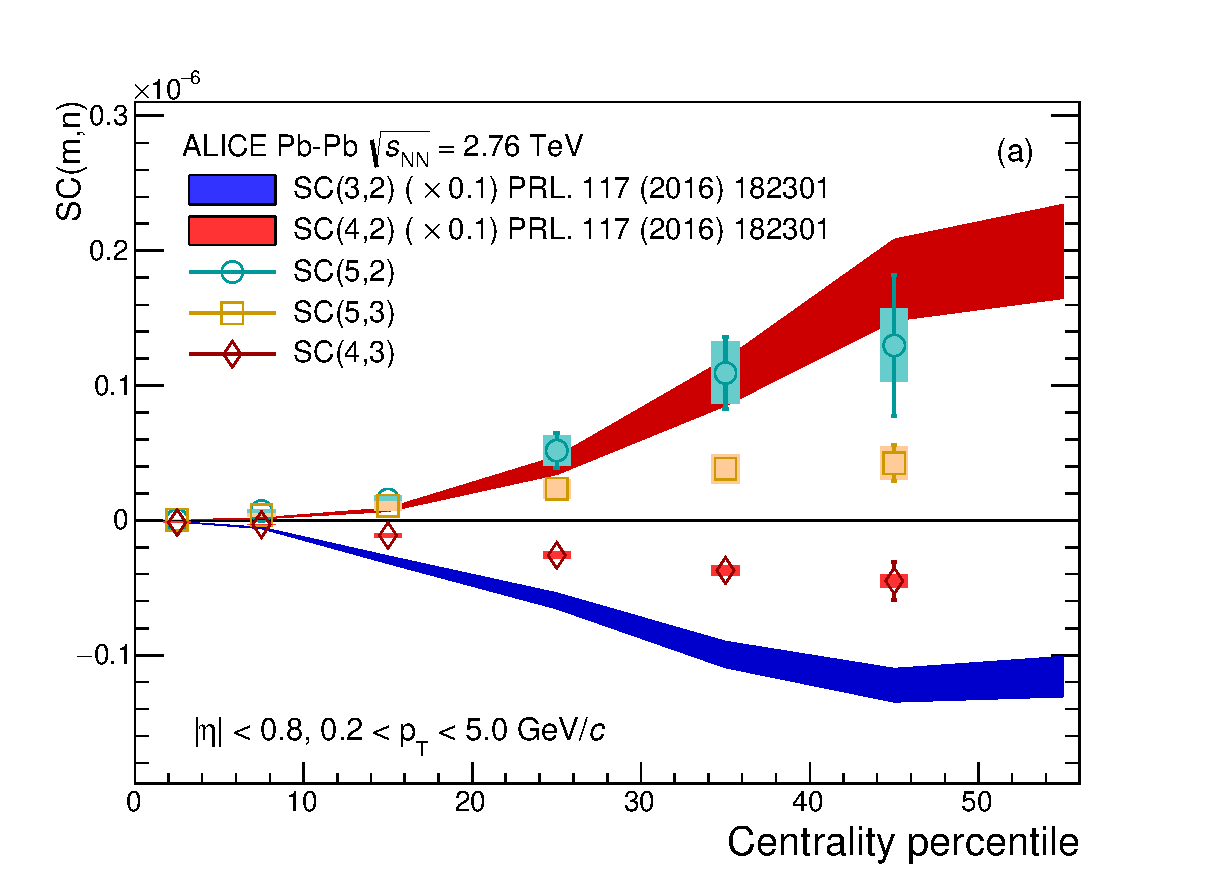
\includegraphics{figs/fig2_QConly_higherSC.eps}}
                       \resizebox{0.48\textwidth}{!}{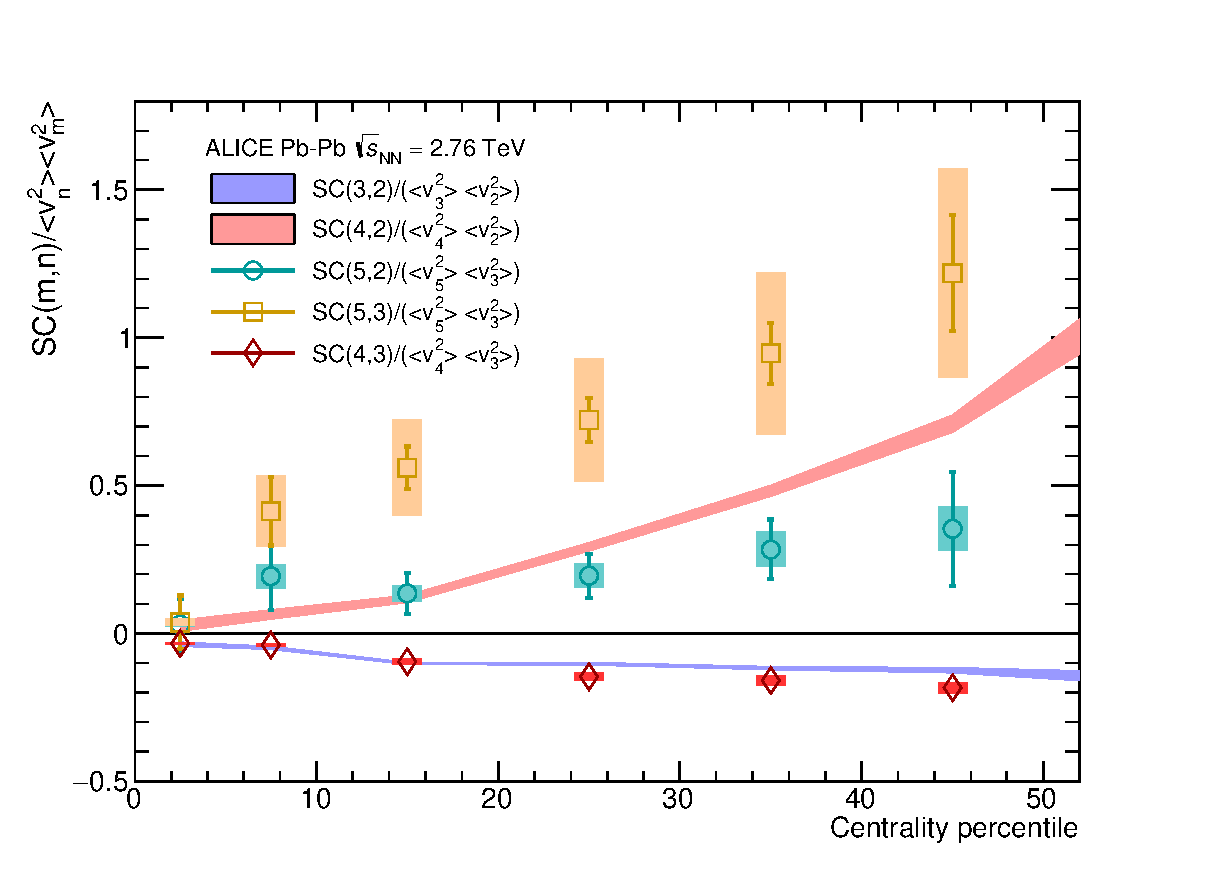
\includegraphics{figs/fig2_QConly_higherNSC.eps}}
        \caption{SC($m$,$n$) (a) and NSC($m$,$n$) (b) with flow harmonics up to $5^{\mathrm{th}}$ order in $\PbPb$ collisions at $\snn=2.76$~TeV. The lower order harmonic correlations (SC(3,2), SC(4,2), NSC(3,2) and NSC(4,2)) are taken from \cite{ALICE:2016kpq} and shown as bands. Note that the systematic and statistical errors are combined in quadrature for these lower order harmonic correlations and SC(4,2) and SC(3,2) are scaled by a factor of 0.1. Systematic errors are represented with boxes.}
        \label{fig:Figure_1}
              \end{center}
\end{figure*}

The higher order flow harmonic correlations (SC(4,3), SC(5,2) and SC(5,3)) are much smaller compared to the lower order harmonic correlations.
In particular SC(5,2) is 10 times smaller than SC(4,2) and SC(4,3) is about 20 times smaller than SC(3,2).

However, unlike SC$(m,n)$, the NSC$(m,n)$ results with the higher order flow harmonics show almost the same order of the correlation strength as the lower order flow harmonic correlations (NSC(3,2) or NSC(4,2)).
The NSC(4,3) magnitude is comparable to NSC(3,2) and one finds that a hierarchy, NSC(5,3) $>$ NSC(4,2) $>$ NSC(5,2), holds for centrality ranges $>$~20\% within the errors as shown in Fig.~\ref{fig:Figure_1}b.
These results indicate that the lower order harmonic correlations are larger than higher order harmonic correlations, not only because of the correlation strength itself but also because of the strength of the individual flow harmonics. 
SC(5,2) is stronger than SC(5,3), but the normalized correlation between $v_5$ and $v_3$ is stronger than the normalized correlation between $v_5$ and $v_2$. 

It can be seen in Fig.~\ref{fig:Figure_1}a that the lower order harmonic correlations as well as SC(5,2) increase non-linearly towards peripheral collisions.
In the case of SC(5,3) and SC(4,3), the centrality dependence is weaker than for the other harmonic correlations.
NSC(5,3) shows the strongest normalized correlation among all harmonics while NSC(5,2) shows the weakest centrality dependence.
Both NSC(3,2) and NSC(4,3) are getting more anticorrelated toward peripheral collisions with the similar magnitude.

\begin{figure*}
	\begin{center}
        	\resizebox{0.42\columnwidth}{!}{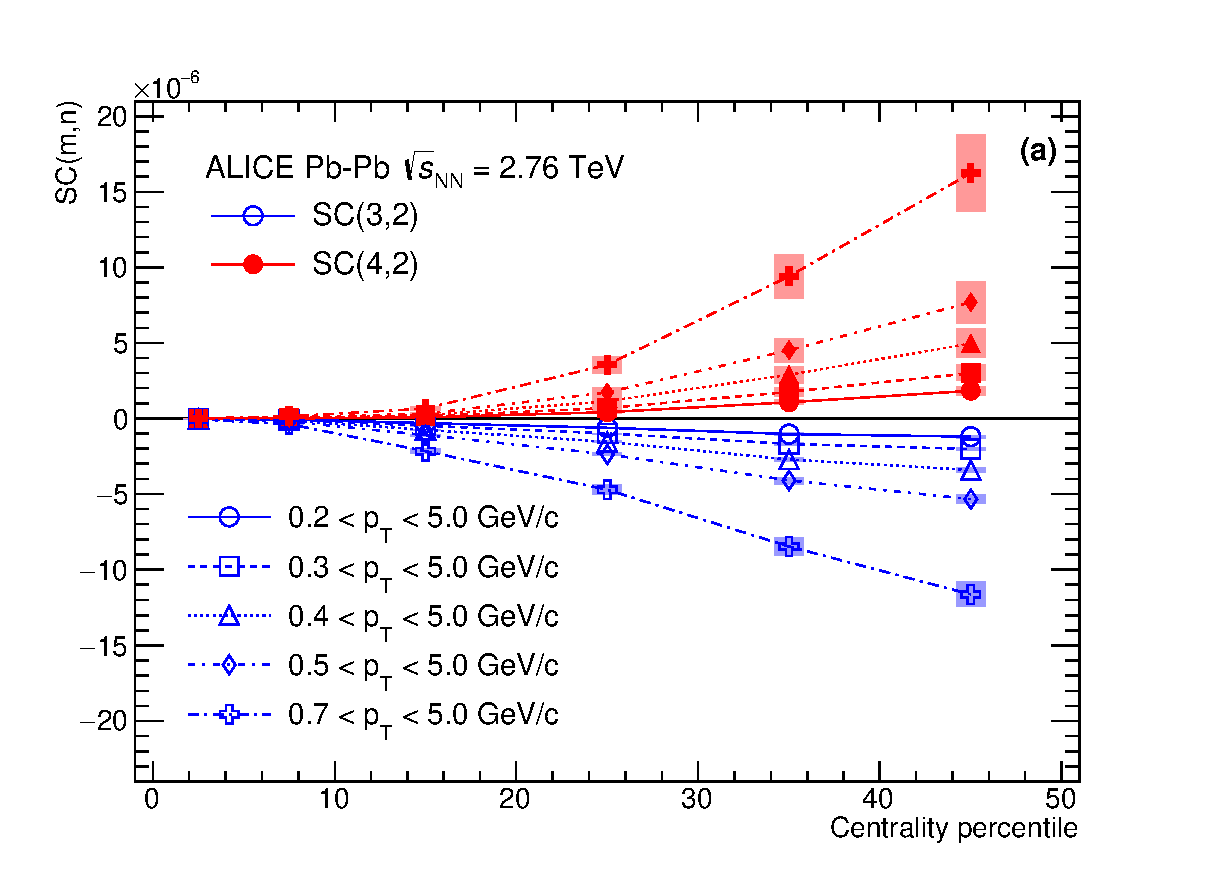
\includegraphics{figs/fig4_QConly_SC_ptdep}}
        	\resizebox{0.42\columnwidth}{!}{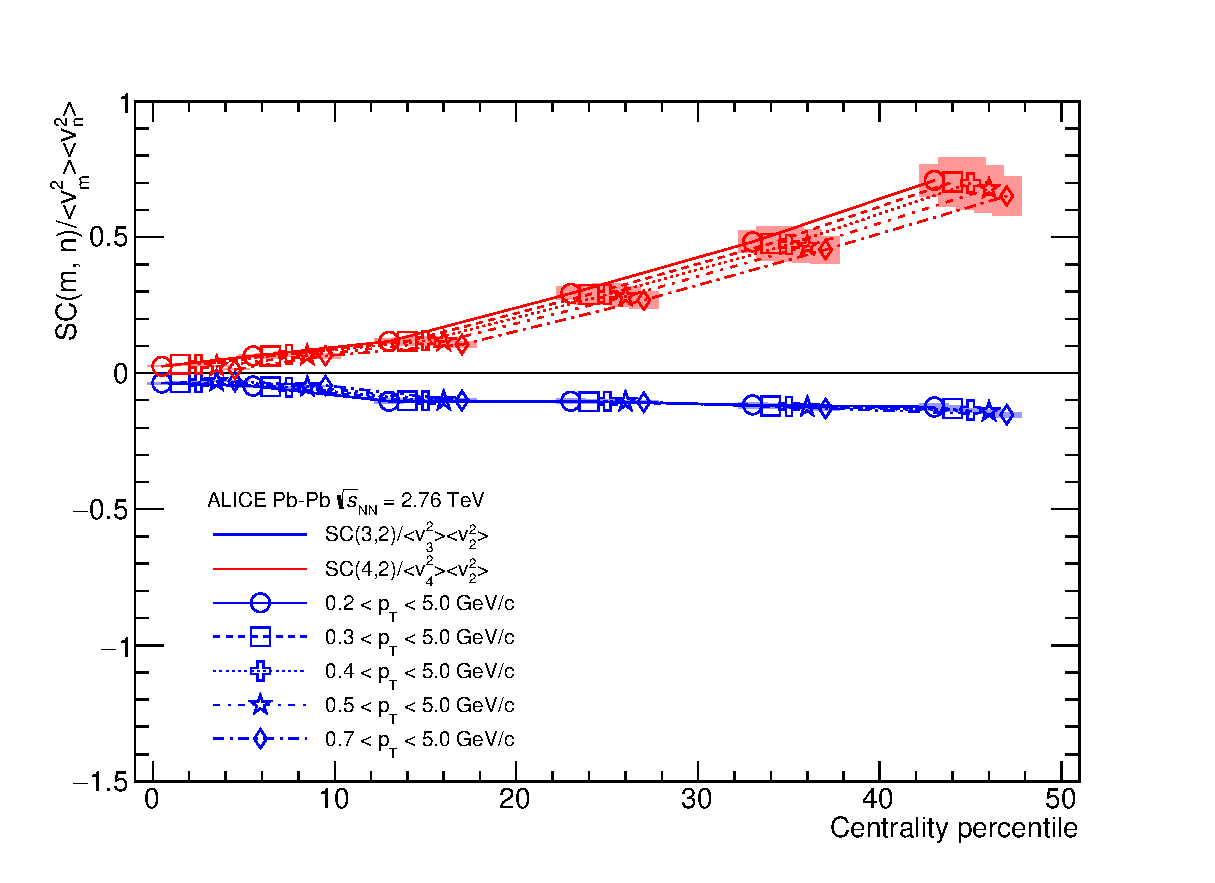
\includegraphics{figs/fig4_QConly_nSC_ptdep}}
	\resizebox{0.42\columnwidth}{!}{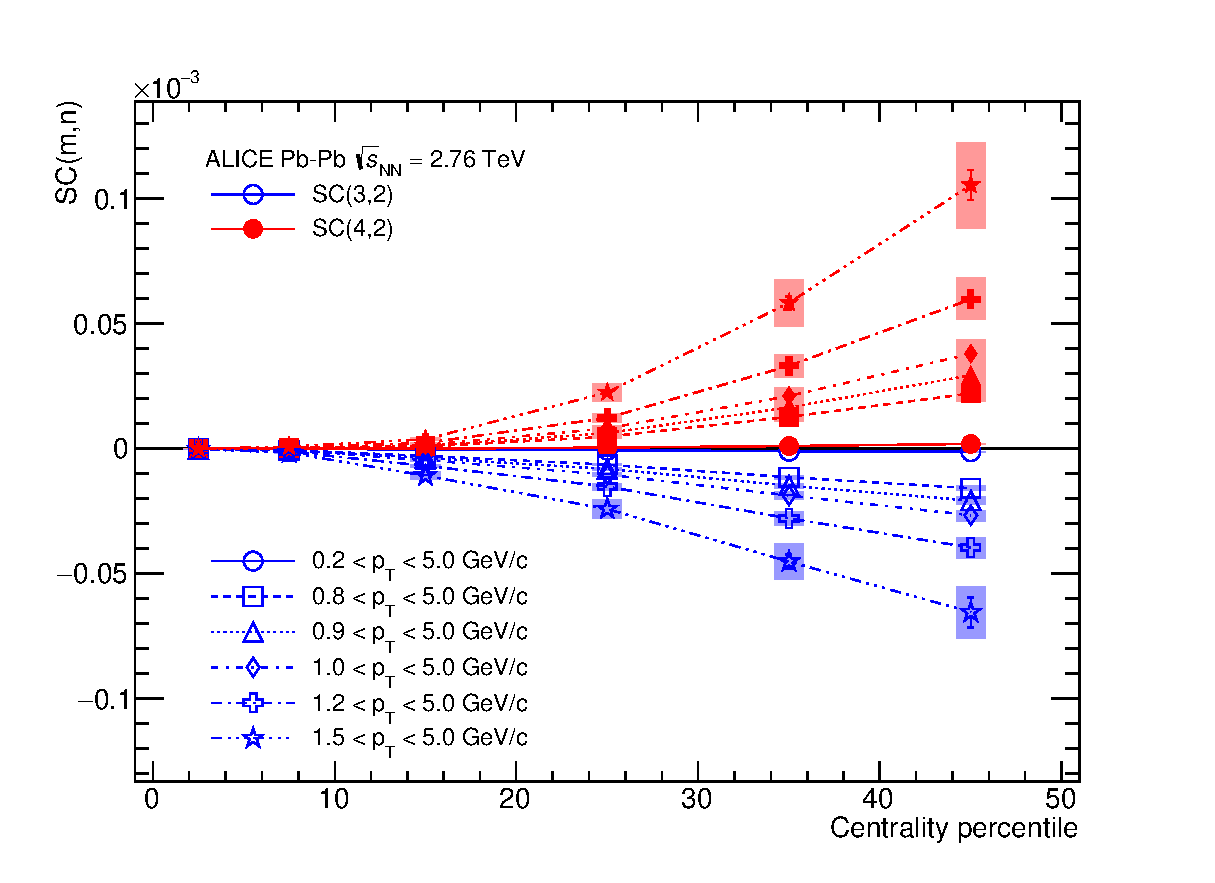
\includegraphics{figs/fig4b_QConly_SC_ptdep}}
        	\resizebox{0.42\columnwidth}{!}{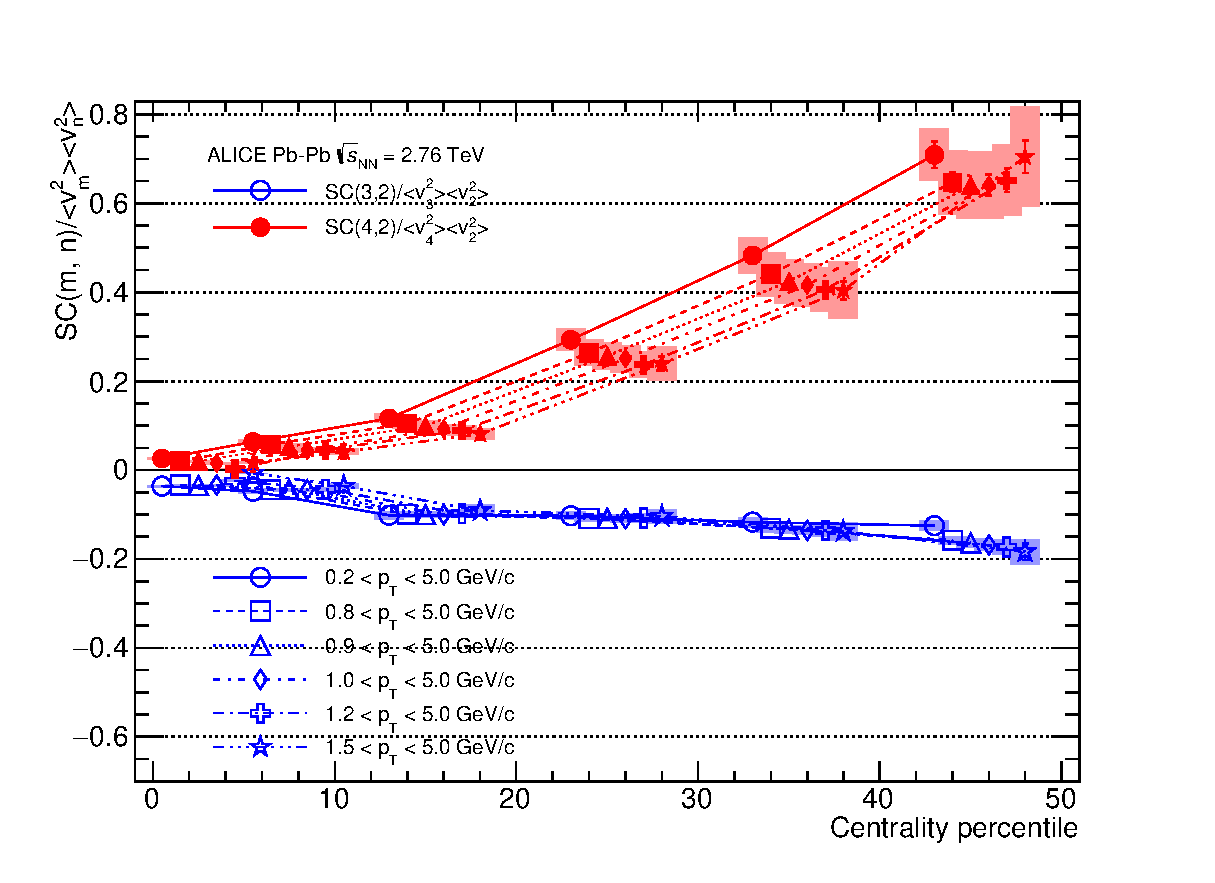
\includegraphics{figs/fig4b_QConly_nSC_ptdep}}
        \caption{SC(3,2) and SC(4,2) with low (a) and high (c) minimum $p_{\rm T}$ cuts, and normalized SC(3,2) and SC(4,2) ((b) and (d)) in $\PbPb$ collisions at $\snn=2.76$~TeV. Panels (a) and (b) show the results for the minimum $p_{\rm T}$ range $0.2<p_{\rm T, min}<0.7$~GeV/$c$ and panels (c) and (d) are for the minimum $p_{\rm T}$ range $0.8<p_{\rm T, min}<1.5$~GeV/$c$. Note that NSC data points from each $p_{\rm T, min}$ in a centrality percentile bin are shifted for visibility.}
        \label{fig:Figure_2}
        \end{center}   
\end{figure*}

To study the $p_{\rm T}$ dependence of SC$(m,n)$, we systematically vary the low $p_{\rm T}$ cut-off ($p_{\rm T, min}$), instead of using independent $p_{\rm T}$ intervals, in order to avoid large statistical fluctuations in the results. Various minimum $p_{\rm T}$ cuts from 0.2 to 1.5~GeV/$c$ are applied.
The $p_{\rm T}$ dependent results for SC(3,2) and SC(4,2) with minimum $p_{\rm T}$ cuts $0.2<p_{\rm T, min}<0.7$~GeV/$c$ are shown in Fig.~\ref{fig:Figure_2}a.
The strength of SC$(m,n)$ becomes larger as $p_{\rm T, min}$ increases. 
%This indicates that the relationship between event-by-event fluctuations of two different flow harmonics $v_m$ and $v_n$ is stronger for high $p_{\rm T}$ particles. 
These $p_{\rm T, min}$ dependent correlations have much stronger centrality dependence, with SC$(m,n)$ getting much larger as centrality or $p_{\rm T, min}$ increases. 
NSC(3,2) and NSC(4,2) with different minimum cuts are shown in Figs.~\ref{fig:Figure_2}b and \ref{fig:Figure_2}d.
The strong $p_{\rm T, min}$ dependence observed in SC$(m,n)$ is not seen in NSC$(m,n)$. The NSC$(m,n)$ results are consistent within the errors for all $p_{\rm T, min}$ cuts. 
This indicates that the $p_{\rm T}$ dependence of SC$(m,n)$ is dominated by the $p_{\rm T}$  dependence of the $\left<v_n\right>$ values. 
The minimum $p_{\rm T}$ cuts are extended from 0.8  to 1.5~GeV/$c$ and the results are shown in Figs.~\ref{fig:Figure_2}c and \ref{fig:Figure_2}d.
While SC$(m,n)$ shows similar trends as for $p_{\rm T, min}<0.8$~GeV/$c$, NSC$(4,2)$ tends to decrease with increasing $p_{\rm T, min}$.
The $p_{\rm T, min}$ dependence of NSC(3,2) is not clearly seen and it is consistent with no $p_{\rm T, min}$ dependence within the statistical and systematic errors for the centrality range $<$~30\%, while showing a moderate decreasing trend with increasing $p_{\rm T, min}$ for the $>$~30\% centrality range.
NSC(4,2) shows a moderate decreasing trend as $p_{\rm T, min}$ increases. These observations are strikingly different from $p_{\rm T}$ dependence of the individual flow harmonics, where the relative flow fluctuations $\sigma_{v_2}/\langle v_{2} \rangle$~\cite{Voloshin:2008dg} are independent of transverse momentum up to $p_{\rm T}$ $\sim$ 8~GeV/$c$ (see Fig. 3 in Ref.~\cite{Abelev:2012di}).
%(see further discussions in Sec.~\ref{sec:ptdepsc})
%This might be an indication of possible viscous corrections for the equilibrium distribution at hadronic freeze-out~\cite{Luzum:2010ad}.
%However within the current statistical and systematic errors, it is consistent with no $p_{\rm T}$ dependence of NSC$(m,n)$ (see further discussions in Sec.~\ref{sec:ptdepsc}).

\section{Model Comparisons}
\label{sec:theory}
%\subsection{Theoretical models}
%\label{sec:models}
%We have used various models in this article. The {\sc HIJING} model~\cite{Wang:1991hta,Gyulassy:1994ew} was utilized to obtain the $p_{\rm T}$-weights~\cite{Bilandzic:2013kga} which were used to estimate systematic bias due to non-uniform reconstruction efficiency as a function of transverse momentum. 
%Secondly, the HIJING model was used to estimate the strength of non-flow correlations (typically few-particle correlations insensitive to the collision geometry). 
%We have evaluated the observables of interest in coordinate space by modeling the initial conditions with a MC-Glauber model~\cite{Miller:2007ri}. 
We have compared the centrality dependence of our observables with event-by-event EKRT+viscous hydrodynamic calculations~\cite{Niemi:2015qia}, where the initial energy density profiles are calculated using a next-to-leading order perturbative-QCD+saturation model~\cite{Paatelainen:2012at,Paatelainen:2013eea}. The subsequent spacetime evolution is described by relativistic dissipative fluid dynamics with different parameterizations for the temperature dependence of the shear viscosity to entropy density ratio $\eta/s(T)$. 
This model gives a good description of the charged hadron multiplicity and the low $p_{\rm T}$ region of the charged hadron spectra at RHIC and the LHC (see Figs.~11-13 in \cite{Niemi:2015qia}).
Each of the $\eta/s(T)$ parameterizations is adjusted to reproduce the measured $v_n$ from central to mid-peripheral collisions (see Fig.~15 in \cite{Niemi:2015qia}). 
%\textbf{Need a short description of event-by-event viscous hydrodynamic calculations from VISH2+1}.

The VISH2+1~\cite{Shen:2010uy,Shen:2014vra} event-by-event calculations for relativistic heavy-ion collisions are based on (2+1)-dimensional viscous hydrodynamics which describes both the QGP phase and the highly dissipative and even off-equilibrium late hadronic stage with fluid dynamics. With well-tuned transport coefficients and decoupling temperature, and given initial conditions discussed later, it can describe the $p_{\rm T}$ spectra and different flow harmonics at RHIC and the LHC~\cite{Qiu:2011hf, Shen:2010uy, Shen:2011eg, Bhalerao:2015iya}.
Three different initial conditions ({MC-Glauber}, {MC-KLN} and {AMPT}) along with different constant $\eta/s$ values are used in the model~\cite{Zhu:2016puf}. 
Traditionally, the Glauber model constructs the initial entropy density with contributions from the wounded nucleon and binary collision density profiles~\cite{Kolb:2000sd}, and the {KLN} model assumes that the initial entropy density is proportional to the initial gluon density calculated from the corresponding $k_{\rm T}$ factorization formula~\cite{Kharzeev:2000ph}. In the Monte Carlo versions ({MC-Glauber} and {MC-KLN})~\cite{Miller:2007ri,Drescher:2006ca,Hirano:2009ah}, additional initial state fluctuations are introduced through position fluctuations of individual nucleons inside the colliding nuclei. For the {AMPT} initial conditions~\cite{Bhalerao:2015iya,Pang:2012he,Xu:2016hmp}, the fluctuating energy density profiles are constructed from the energy decompositions of individual partons, which fluctuate in both momentum and position coordinate. Compared with the {MC-Glauber} and {MC-KLN} initial conditions, the additional Gaussian smearing in the {AMPT} initial conditions gives rise to non-vanishing initial local flow velocities~\cite{Pang:2012he}.
%The AMPT initial conditions is basically HIJING with the location of the strings specified according to the sites of the nucleon nucleon collisions. The model then introduces the string melting procedure to produce initial partons. These partons are then evolved for the short duration using the ZPC parton cascade model. Instead the initial energy momentum tensor is directly fed into the hydrodynamic calculations, the energy density and the flow velocity are first obtained using the Landau condition and only the ideal fluid parts are used as the initial condition for the hydrodynamic evolution. Mini-jets from semi-hard parton scatterings are assumed to be locally thermalized through a Gaussian smearing and give rise to non-vanishing initial local flow velocities~\cite{Pang:2012he}.

The centrality dependence of the SC observables is compared to that in the {AMPT} model~\cite{Zhang:1999bd,Lin:2000cx,Lin:2004en}.
Even though thermalization could be achieved in collisions of very large nuclei and/or at extremely high energy~\cite{Kurkela:2015qoa}, the dense matter created in heavy-ion collisions may not reach full thermal or chemical equilibrium as a result of its finite volume and short lifetime. To address such non-equilibrium many-body dynamics, AMPT has been developed, which includes both initial partonic and final hadronic interactions and the transition between these two phases of matter.
For the initial conditions, the AMPT model uses the spatial and momentum distributions of hard minijet partons and soft strings from the HIJING model~\cite{Wang:1991hta,Gyulassy:1994ew}.
The AMPT model can be run in two main configurations, the default and the string melting model~\footnote{The input parameters used in both configurations are: $\alpha_s = 0.33$, a partonic cross-section of 1.5~mb, while the Lund string fragmentation parameters were set to $\alpha = 0.5$ and $b = 0.9$~GeV$^{-2}$.}.
In the default version, partons are recombined with their parent strings when they stop interacting. The resulting strings are later converted into hadrons using the Lund string fragmentation model~\cite{Andersson:1986gw,NilssonAlmqvist:1986rx}. In the string melting version, the initial strings are melted into partons whose interactions are described by the ZPC parton cascade model~\cite{Zhang:1997ej}. These partons are then combined into the final state hadrons via a quark coalescence model. 
In both configurations, the dynamics of the subsequent hadronic matter is described by a hadronic cascade based on A Relativistic Transport (ART) model~\cite{Li:2001xh} which also includes resonance decays.
The third version used in this article is based on the string melting configuration in which the hadronic rescattering phase is switched off to study its influence on the development of anisotropic flow. 
Even though the string melting version of AMPT~\cite{Lin:2001zk,Lin:2004en} reasonably reproduces particle yields, $p_{\rm T}$ spectra, and $v_2$ of low $p_{\rm T}$ pions and kaons in central and mid-central $\AuAu$ collisions at $\snn=200$~GeV and $\PbPb$ collisions at $\snn=2.76$~TeV~\cite{Lin:2014tya}, it was seen clearly in a recent study~\cite{Adam:2016nfo} that it fails to quantitatively reproduce the flow coefficients of identified hadrons ($v_2$, $v_3$, $v_4$ and $v_5$) at $\snn=2.76$~TeV. It turns out that the radial flow in AMPT is 25\% lower than that measured at the LHC, which is responsible for the quantitative disagreement~\cite{Adam:2016nfo}. The details of the AMPT configurations used in this article and the comparisons of $p_{\rm T}$-differential $v_{n}$ for pions, kaons and protons to the data can be found in \cite{Adam:2016nfo}.

%Two mechanisms in {AMPT} produce collective effects: partonic and hadronic rescattering. Before partonic rescattering, the initially produced strings may be broken into smaller pieces by the %so-called string melting. Three different {AMPT} settings are considered, having either string melting or hadronic rescattering or both activated.

\subsection{Low Order Harmonic Correlations}
\label{sec:theory_loworder}
SC(3,2) and SC(4,2) are compared to several theoretical calculations. 
The event-by-event EKRT+viscous hydrodynamic predictions with the different parameterizations for the temperature dependence of the shear viscosity to entropy density ratio $\eta/s(T)$ are shown in Fig.~2 of Ref.~\cite{ALICE:2016kpq}. 
In this previous work it was demonstrated that NSC(3,2) is sensitive mainly to the initial conditions, while NSC(4,2) is sensitive to both the initial conditions and the system properties, which is consistent with the predictions from~\cite{Niemi:2012aj}.
However, the sign of NSC(3,2) is negative in the data in 0--10\% central collisions while it is positive in the models where the anisotropies originate mainly from fluctuations.
This observation helps us to better understand the fluctuations in initial energy density.
NSC(4,2) shows better sensitivity for different $\eta/s(T)$ parameterizations but the model cannot describe either the centrality dependence or the absolute values. This observed discrepancy between data and theoretical predictions indicates that the current understanding of initial conditions in models of heavy-ion collisions needs to be revisited to further constrain $\eta/s(T)$.
%, considering the difficulties in separating the role of $\eta/s$ from the initial conditions to the final state particle anisotropies~\cite{Romatschke:2007mq,Shen:2011zc}.
The measurement of SC$(m,n)$ and NSC$(m,n)$ can provide new constraints for the detailed modeling of fluctuating initial conditions. Better constraints on the initial state conditions will certainly reduce the uncertainties in determining $\eta/s(T)$.
 
The comparison to the VISH2+1 calculation~\cite{Zhu:2016puf} is shown in Fig.~\ref{fig:Figure_3}.  All calculations with large $\eta/s$ regardless of the initial conditions ($\eta/s=0.2$ for MC-KLN and MC-Glauber initial conditions and $\eta/s=0.16$ for AMPT initial conditions) fail to capture the centrality dependence of SC(3,2) and SC(4,2). 
Among the calculations with small $\eta/s$ ($\eta/s=0.08$), the one with the AMPT initial conditions describes the data better both for SC(3,2) and SC(4,2) but it cannot describe the data quantitively for most of the centrality ranges.
Similar to the event-by-event EKRT+viscous hydrodynamic calculations~\cite{Niemi:2015qia}, the sign of the normalized NSC(3,2) in the model calculations in Fig.~\ref{fig:Figure_3} is opposite to that in data in 0--10\% central collisions. NSC(3,2) does not show sensitivity to the initial conditions nor to the different $\eta/s$ parameterizations used in the models and cannot be described quantitatively by these models.
However, NSC(4,2) is sensitive both to the initial conditions and the $\eta/s$ parameterizations used in the models.
Even though NSC(4,2) favors both AMPT initial conditions with $\eta/s=0.08$ and MC-Glauber initial conditions with $\eta/s=0.20$,
SC(4,2) can only be described by models with smaller $\eta/s$. Hence the calculation with large $\eta/s=0.20$ is ruled out. We conclude that $\eta/s$ should be small and that AMPT initial conditions are favored by the data.

\begin{figure*}[!]
	\begin{center}
        	\resizebox{0.40\columnwidth}{!}{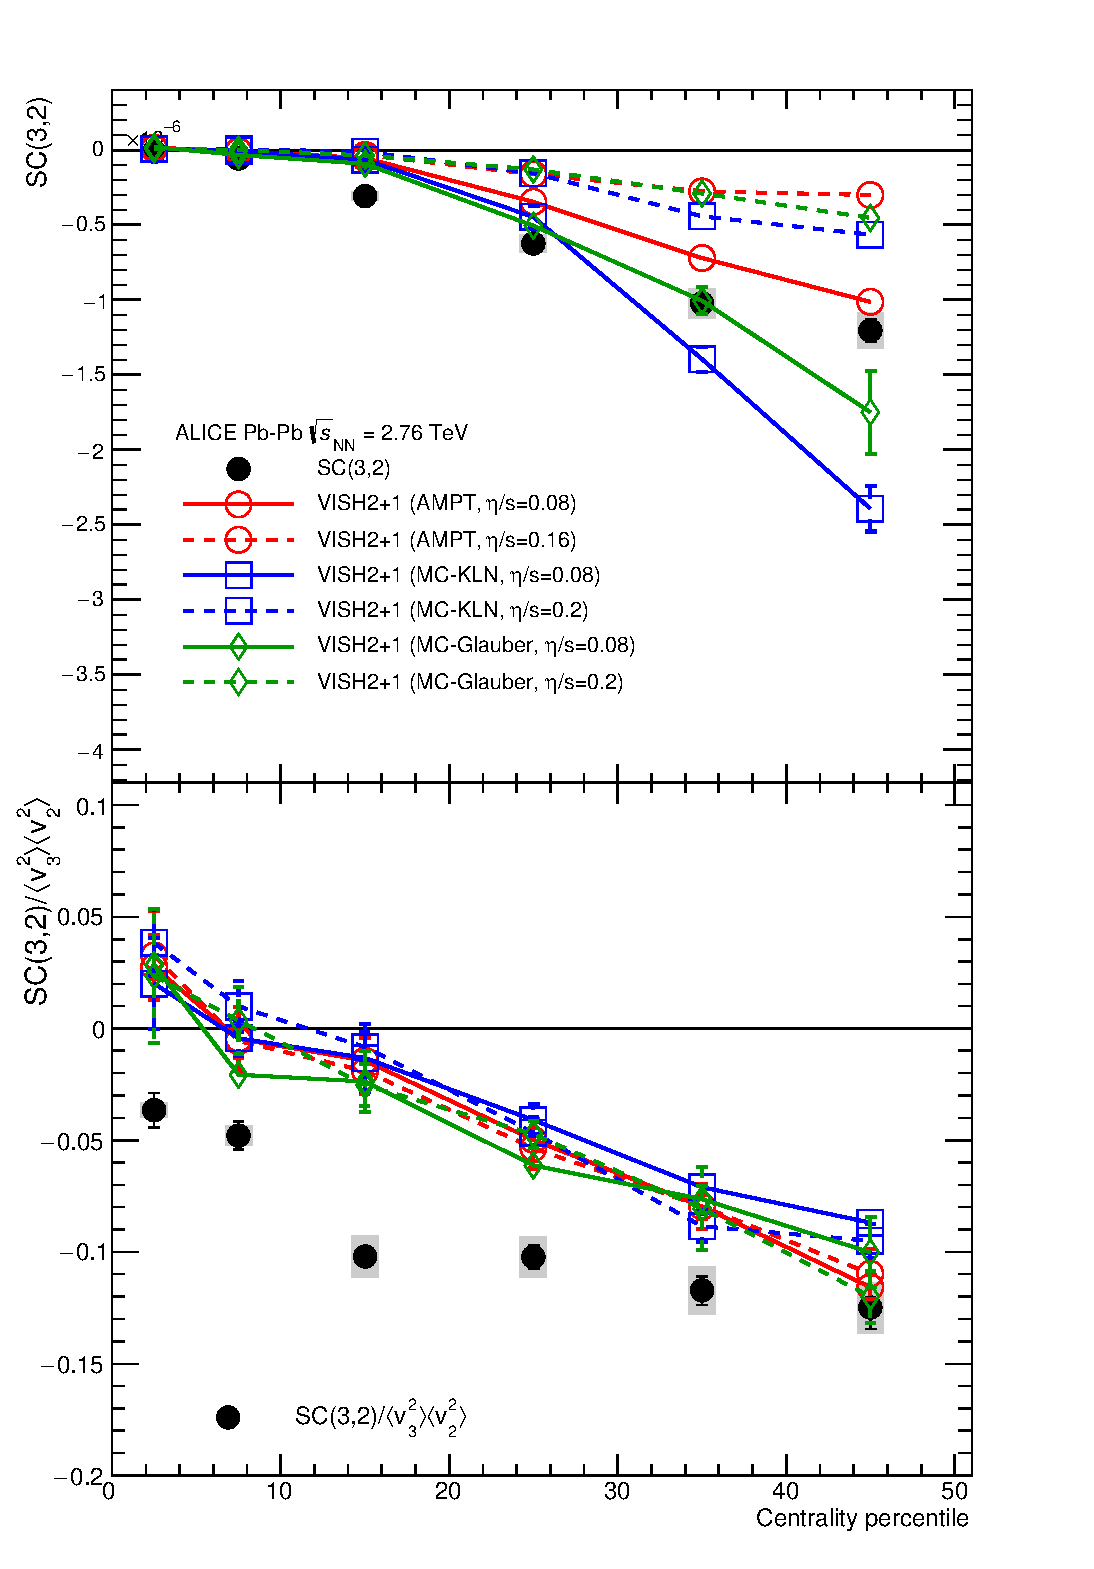
\includegraphics{figs/fig3_QConly_ModelComparison_SC32_vish.eps}}
        	\resizebox{0.40\columnwidth}{!}{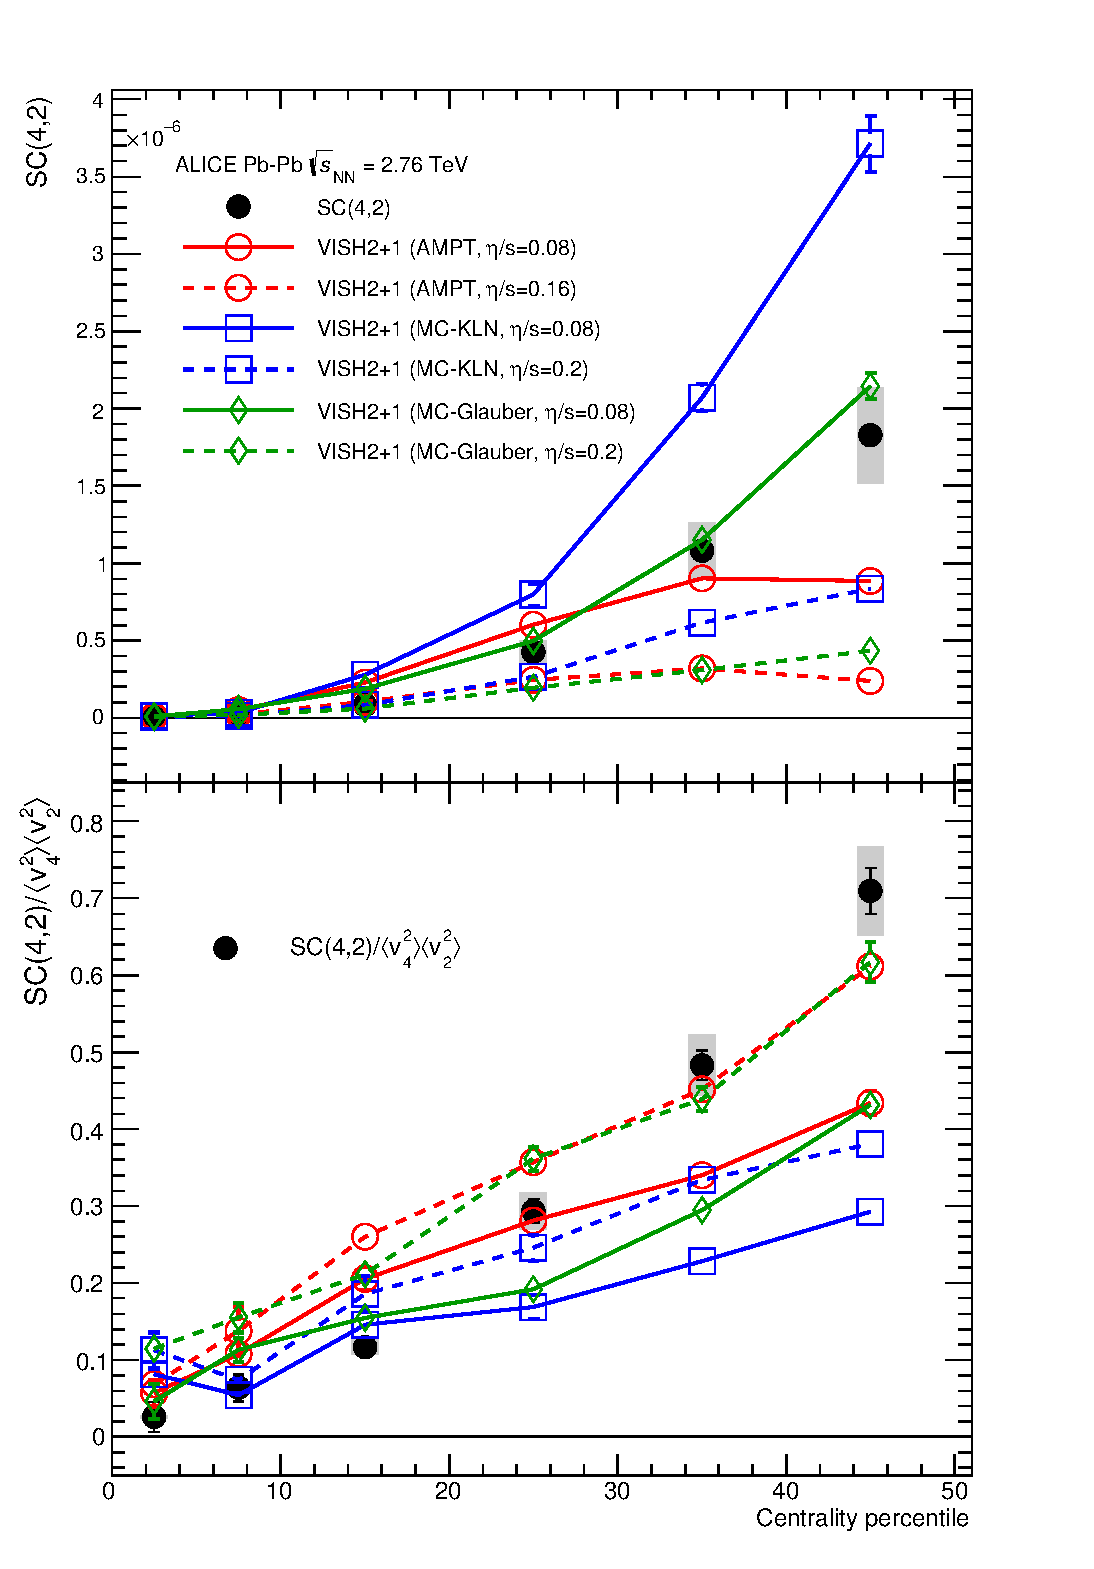
\includegraphics{figs/fig3_QConly_ModelComparison_SC42_vish.eps}}
        \caption{SC(3,2) (a) and SC(4,2) (b) in $\PbPb$ collisions at $\snn=2.76$~TeV are compared to various VISH2+1 calculations~\cite{Zhu:2016puf} with different settings. Upper (lower) panels show SC($m$,$n$) (NSC($m$,$n$)).
        Calculations with AMPT, MC-KLN, and MC-Glauber initial conditions are drawn as different colors and markers. The $\eta/s$ parameters are shown in different line styles, the small $\eta/s=0.08$ are shown as solid lines, and large $\eta/s$~(0.2 for MC-KLN and MC-Glauber, 0.16 for AMPT) are drawn as dashed lines. }
         \label{fig:Figure_3}
        \end{center}   
 \end{figure*}
 
\begin{figure*}[!]
	\begin{center}
        	\resizebox{0.40\columnwidth}{!}{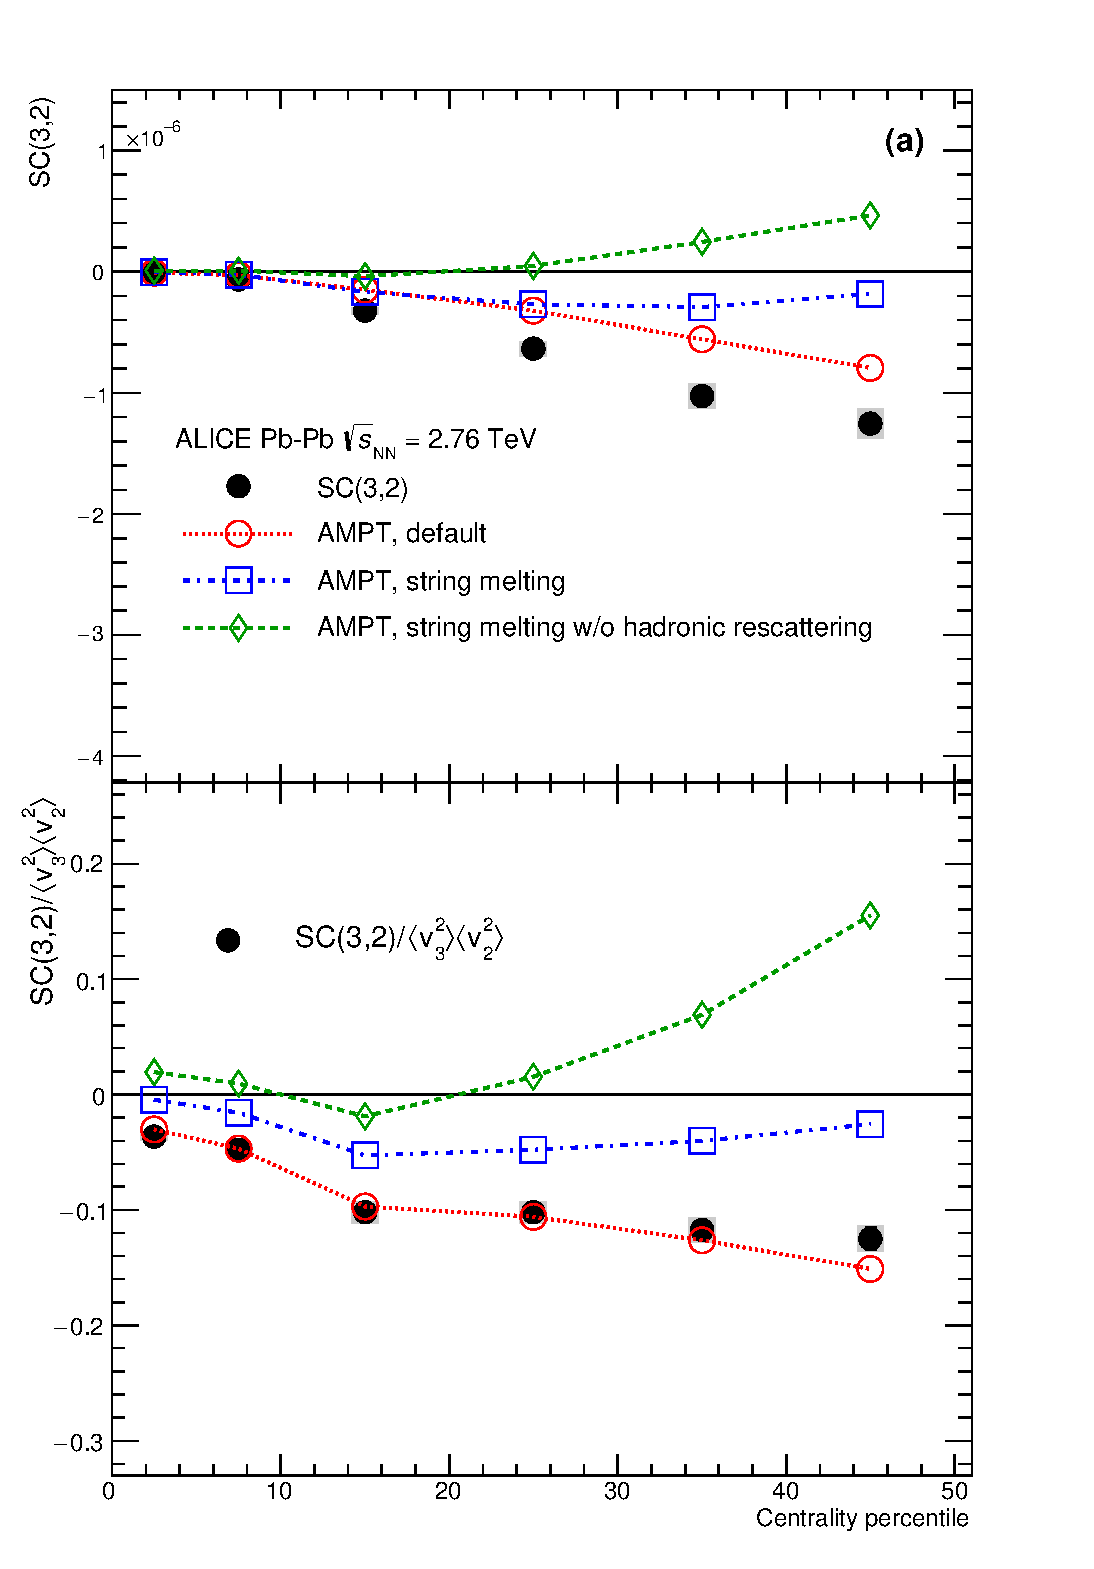
\includegraphics{figs/fig3_QConly_ModelComparison_SC32_ampt.eps}}
        	\resizebox{0.40\columnwidth}{!}{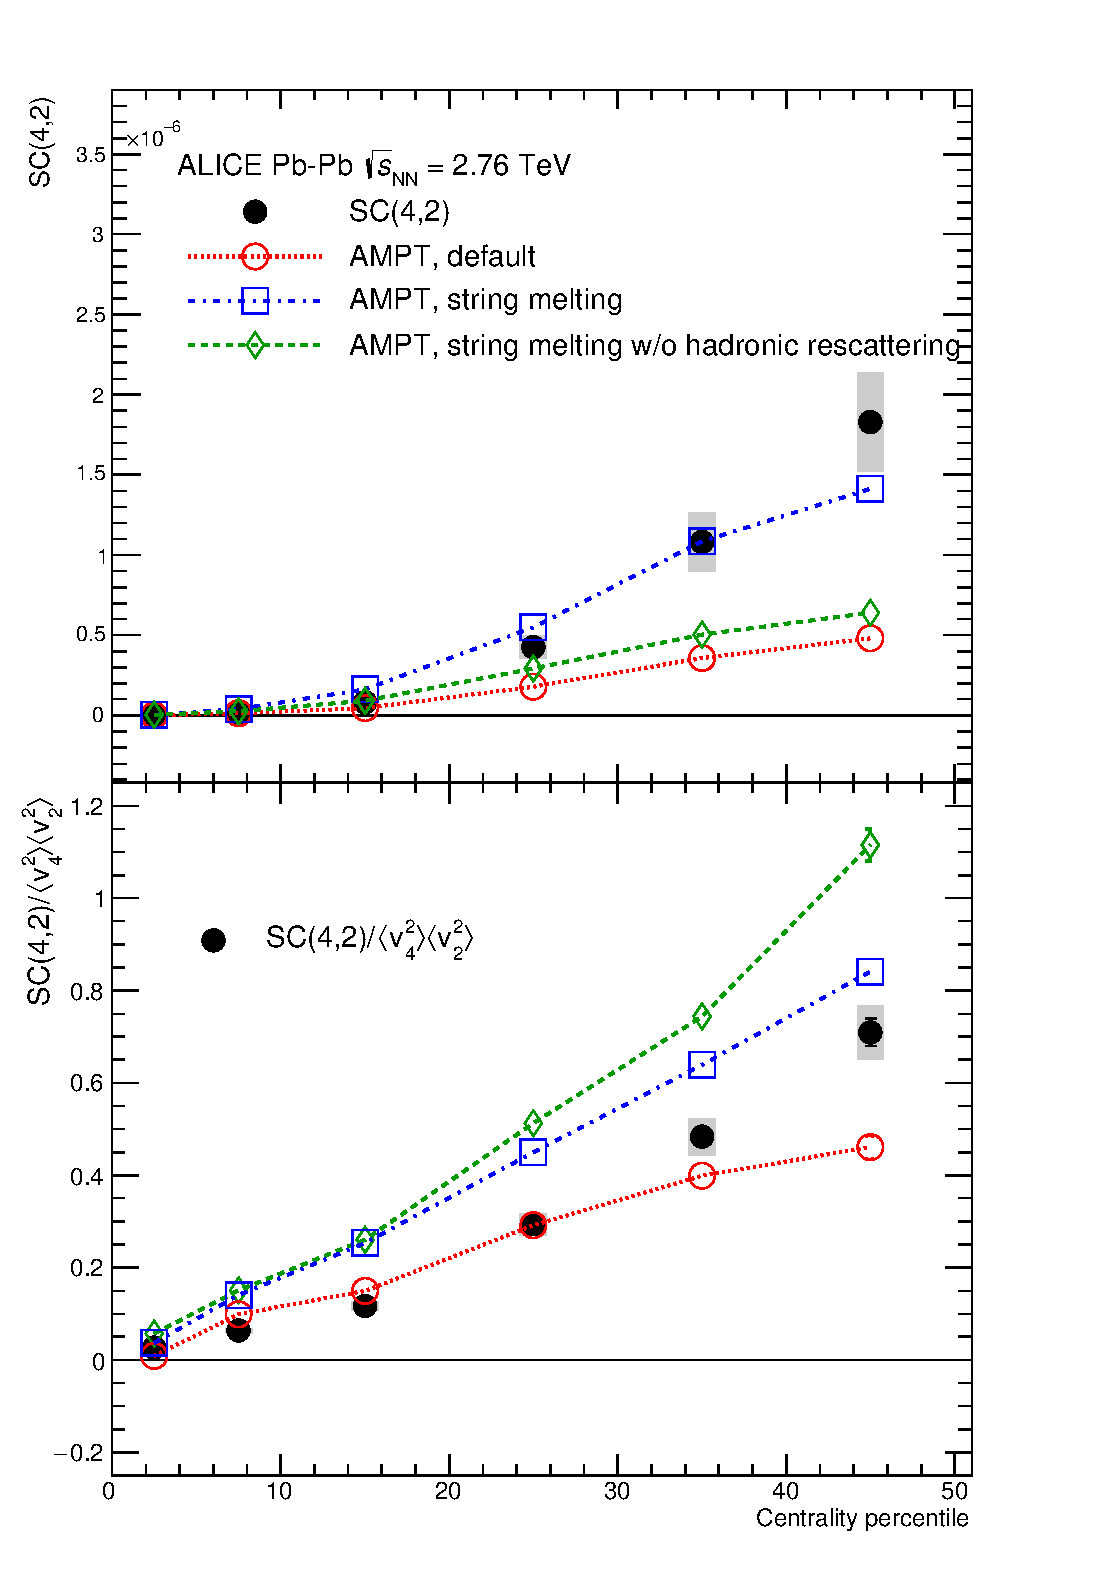
\includegraphics{figs/fig3_QConly_ModelComparison_SC42_ampt.eps}}
        \caption{SC(3,2) (a) and SC(4,2) (b) in $\PbPb$ collisions at $\snn=2.76$~TeV are compared to various AMPT models. Upper (lower) panels show SC$(m,n)$ (NSC$(m,n)$).}
        \label{fig:Figure_4}
        \end{center}   
 \end{figure*}
 
SC($m$,$n$) calculated from AMPT simulations are compared with data in Fig.~\ref{fig:Figure_4}.
For SC(3,2), the calculation with the default AMPT settings is closest to the data, but none of the AMPT configurations can describe the data fully. 
The same default calculation can describe the sign and magnitude of NSC(3,2) while the hydrodynamic calculations fail to describe either of them in the most central collisions.
Interestingly, the string melting AMPT configuration cannot reproduce the data, and the resulting correlations are weaker than in data.
The third version based on the string melting configuration without the hadronic rescattering phase is also shown.
The hadronic rescattering stage makes both SC(3,2) and NSC(3,2) stronger in the string melting AMPT model but not enough to describe the data.
Further investigations proved why the default AMPT model can describe NSC(3,2) fairly well but underestimates SC(3,2). By taking the differences in the individual flow harmonics ($v_2$ and $v_3$) between the model and data into account, it was possible to recover the difference in SC(3,2) between the data and the model. The discrepancy in SC(3,2) can be explained by the overestimated individual $v_n$ values as reported in \cite{Adam:2016nfo} in all centrality ranges. 

In the case of SC(4,2), the string melting AMPT model can describe the data fairly well while the default model underestimates it.
NSC(4,2) is slightly overestimated by the string melting setting which can describe SC(4,2) but the default AMPT configuration can describe the data better.
The influence of the hadronic rescattering phase on NSC(4,2) is opposite to other observables (SC(3,2), NSC(3,2) and SC(4,2)). The hadronic rescattering makes NSC(4,2) slightly smaller.
It should be noted that the agreement with SC$(m,n)$ should not be overemphasized since there are discrepancies in the individual $v_n$ between the AMPT models and the data as was demonstrated for SC(3,2).
Hence the simultaneous description of SC$(m,n)$ and NSC$(m,n)$ should give better constraints on the parameters in AMPT models.

\subsection{Higher Order Harmonic Correlations}
\label{sec:theory_highorder}
The higher order harmonic correlations (SC(4,3), SC(5,2) and SC(5,3)) are compared to several theoretical model calculations. 
The event-by-event EKRT+viscous hydrodynamic predictions with the different parameterizations for the temperature dependence of the shear viscosity to entropy density ratio $\eta/s(T)$ are shown in Fig.~\ref{fig:Figure_5}. 
While we discussed the comparison to these hydrodynamic model calculations with various temperature dependent $\eta/s$ parameterizations, only two calculations with the parameters which describe the lower order harmonic correlations best are compared to the results of higher order harmonic correlations. 
As can be seen in Fig.~1 from Ref.~\cite{Niemi:2015qia}, for ``param1'' parameterization the phase transition from the hadronic to the QGP phase occurs at the lowest temperature, around 150~MeV. This parameterization is also characterized by a moderate slope in $\eta/s(T)$ which decreases (increases) in the hadronic (QGP) phase.
The model calculations in which the temperature of the phase transition is larger than for the ``param1'' can be ruled out by the previous measurements~\cite{ALICE:2016kpq}.
As shown in Fig.~\ref{fig:Figure_5}, only the correlations between $v_5$ and $v_2$ are well described for all available centralities. 
On the other hand, for correlations between $v_5$ and $v_3$ the description fails in more peripheral collisions, providing further independent constraints for the models.
%The model calculations for SC(5,2) and SC(5,3) give better description than the correlations between $v_4$ and $v_2$. 
In the case of the correlation between $v_4$ and $v_3$, the same models underestimate the anticorrelation in the data significantly.
Most notably, this measurement is so far the most dramatic example of the failure of constant $\eta/s$ to describe the data.

%\begin{figure*}[!]
%            \begin{center}
%                       \resizebox{0.32\textwidth}{!}{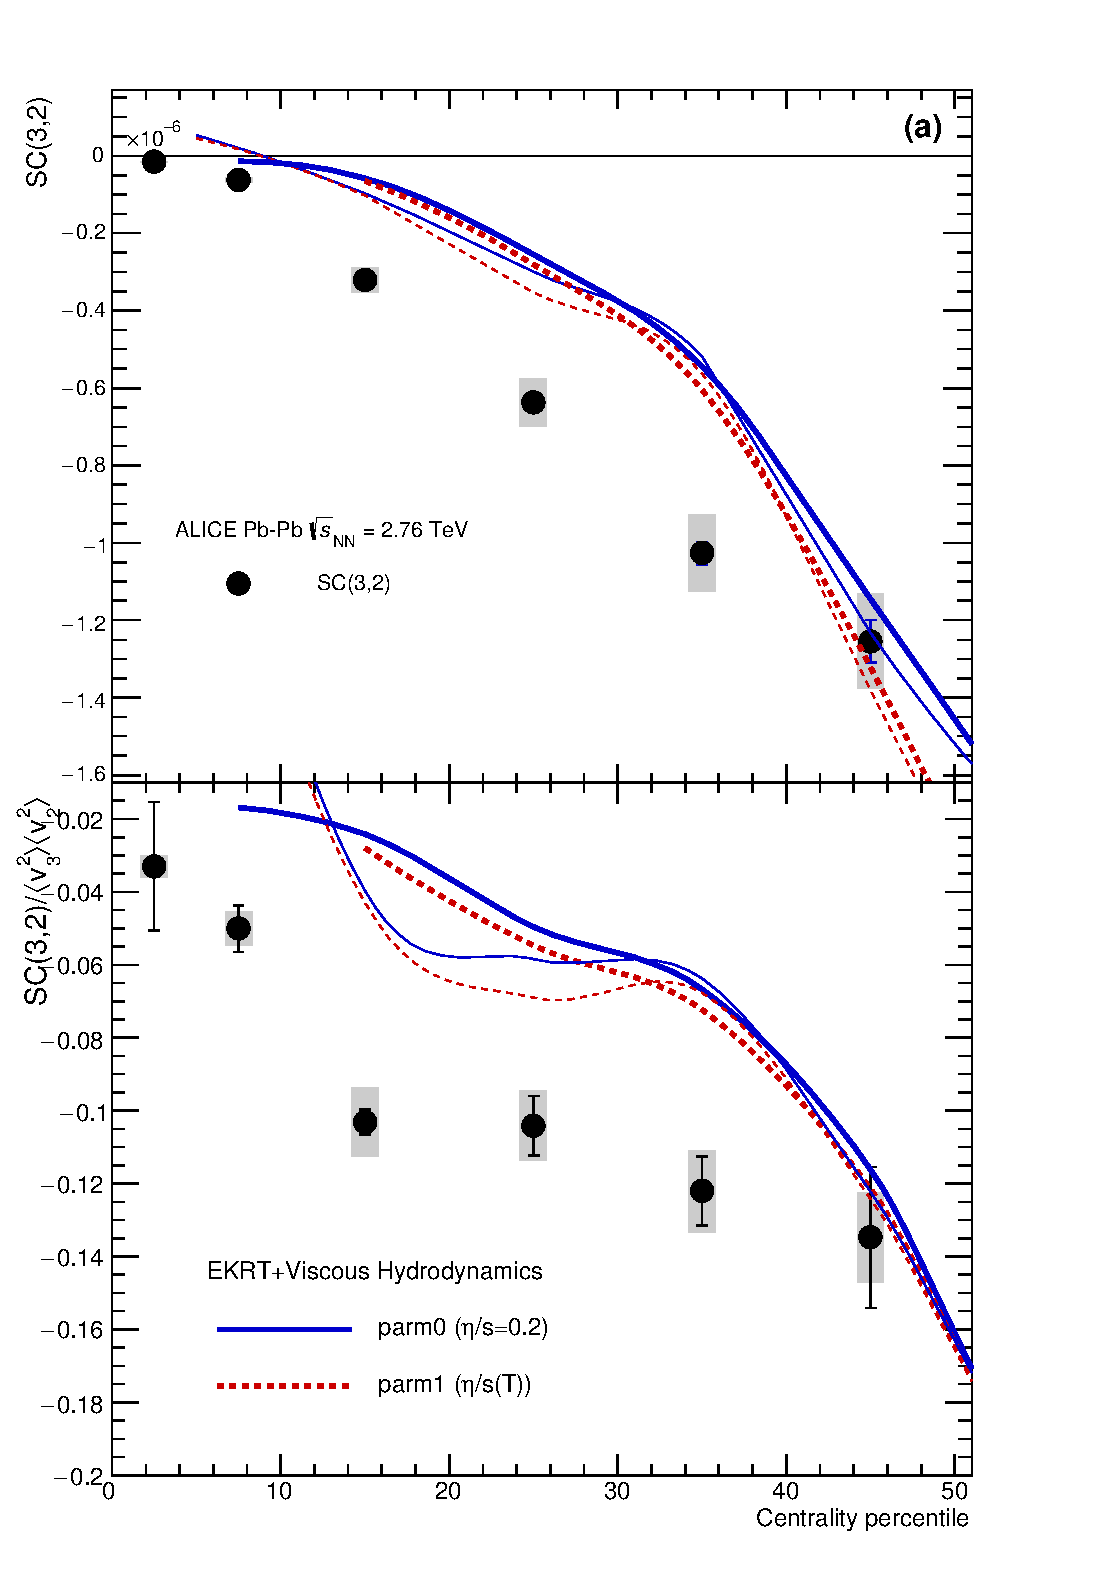
\includegraphics{figs/fig3_QConly_ModelComparison_SC32_EKRT_backup.eps}}
%                       \resizebox{0.32\textwidth}{!}{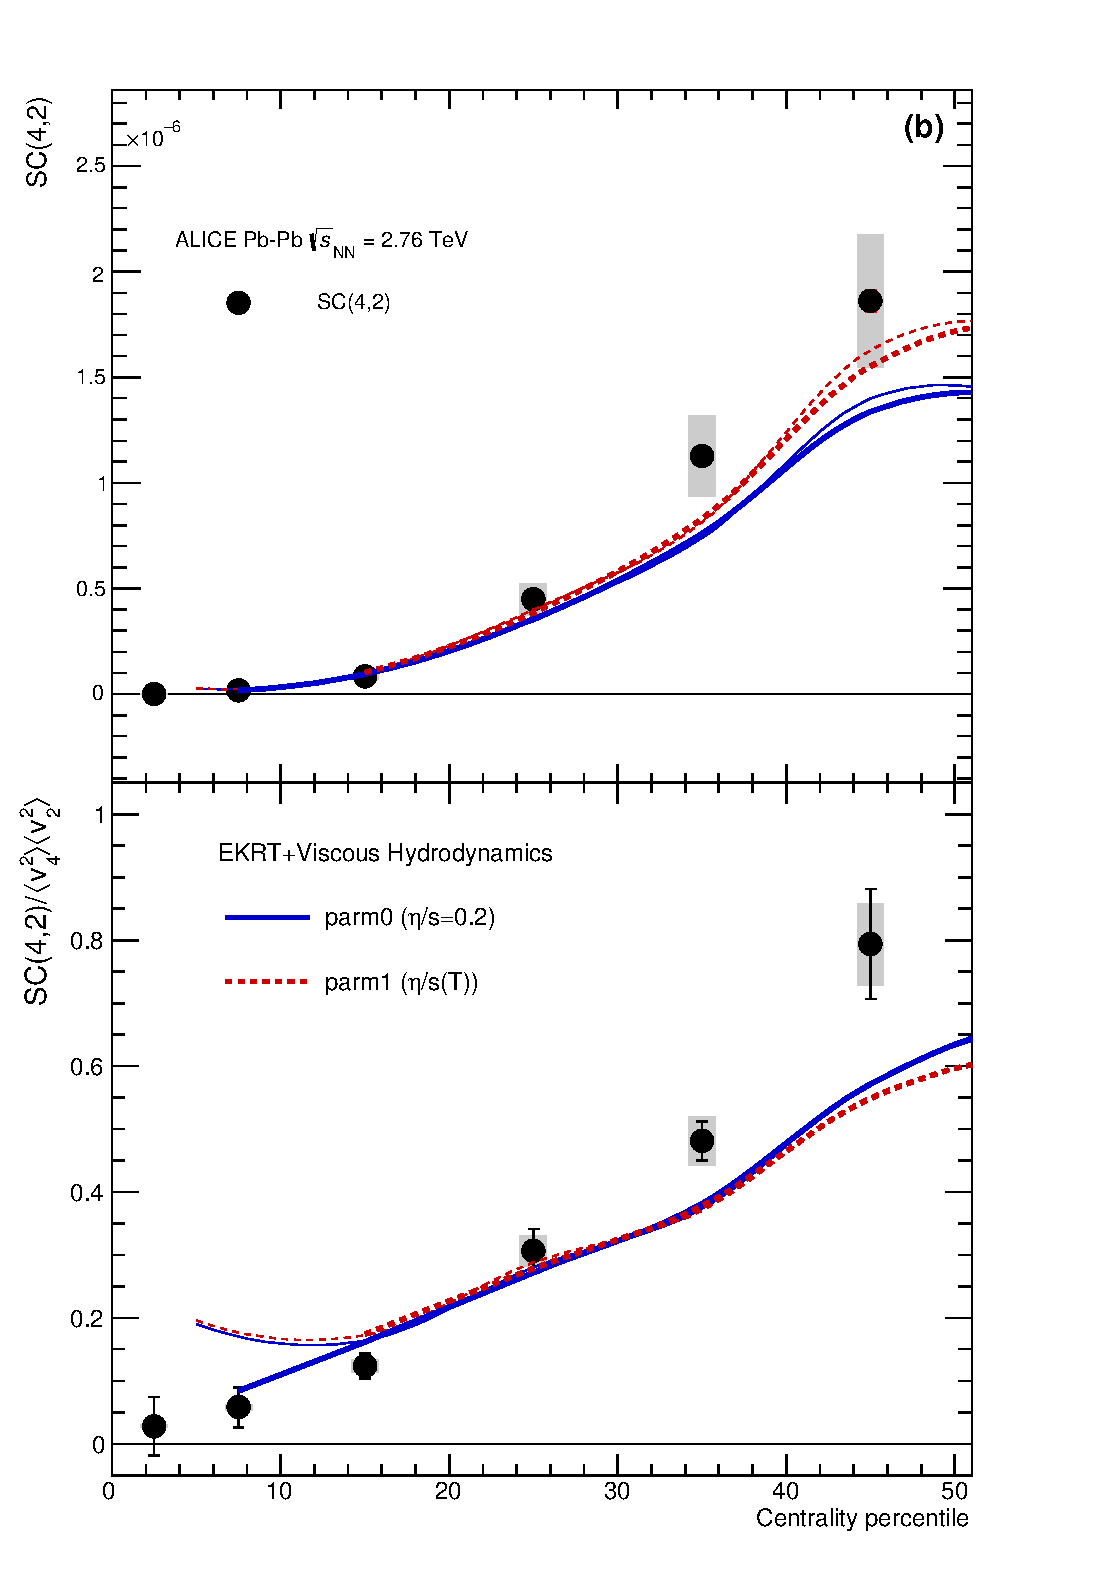
\includegraphics{figs/fig3_QConly_ModelComparison_SC42_EKRT_backup.eps}}
%                \end{center}
%        \caption{Measurements of  SC(3,2) and SC(4,2) in $\PbPb$ collisions at $\snn=2.76$~TeV are compared to the event-by-event EKRT+viscous hydrodynamic calculations~\cite{Niemi:2015qia}. The lines are hydrodynamic predictions with $\eta/s(T)$ parameterizations~\cite{Niemi:2015qia}.}
%        \label{fig:Figure_5_0}
%\end{figure*}
%

\begin{figure*}[!]
            \begin{center}
                       \resizebox{0.32\textwidth}{!}{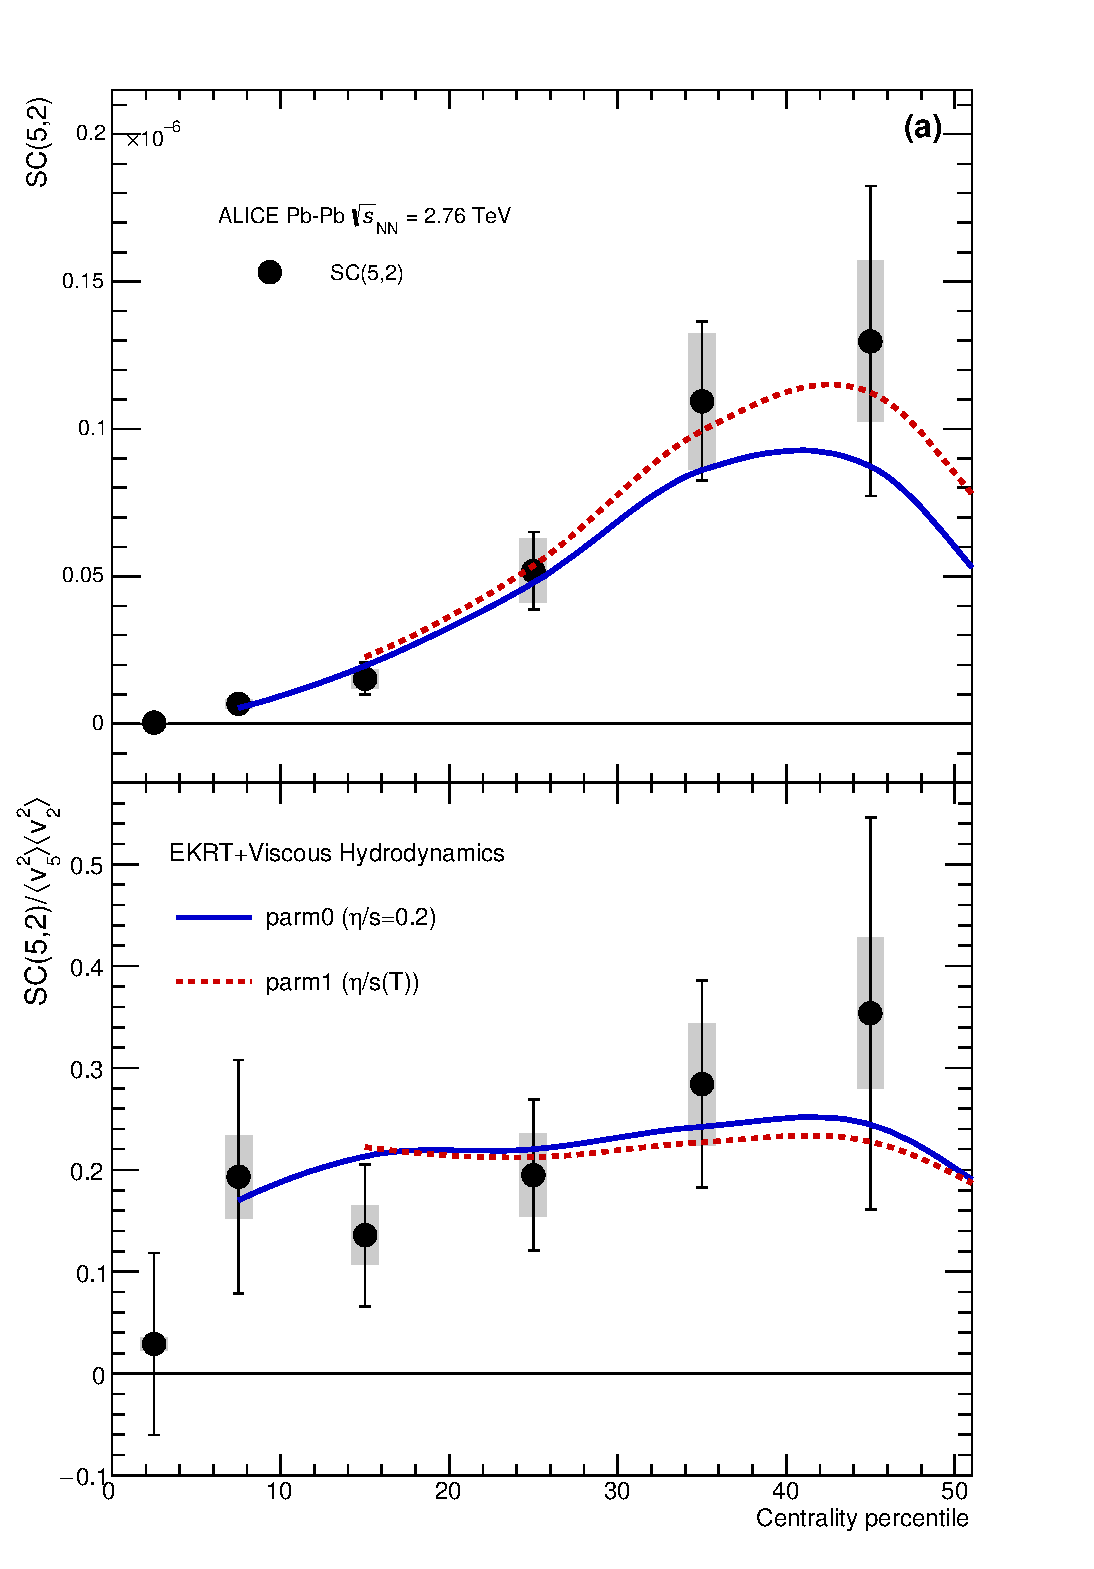
\includegraphics{figs/fig3_QConly_ModelComparison_SC52_EKRT.eps}}
                       \resizebox{0.32\textwidth}{!}{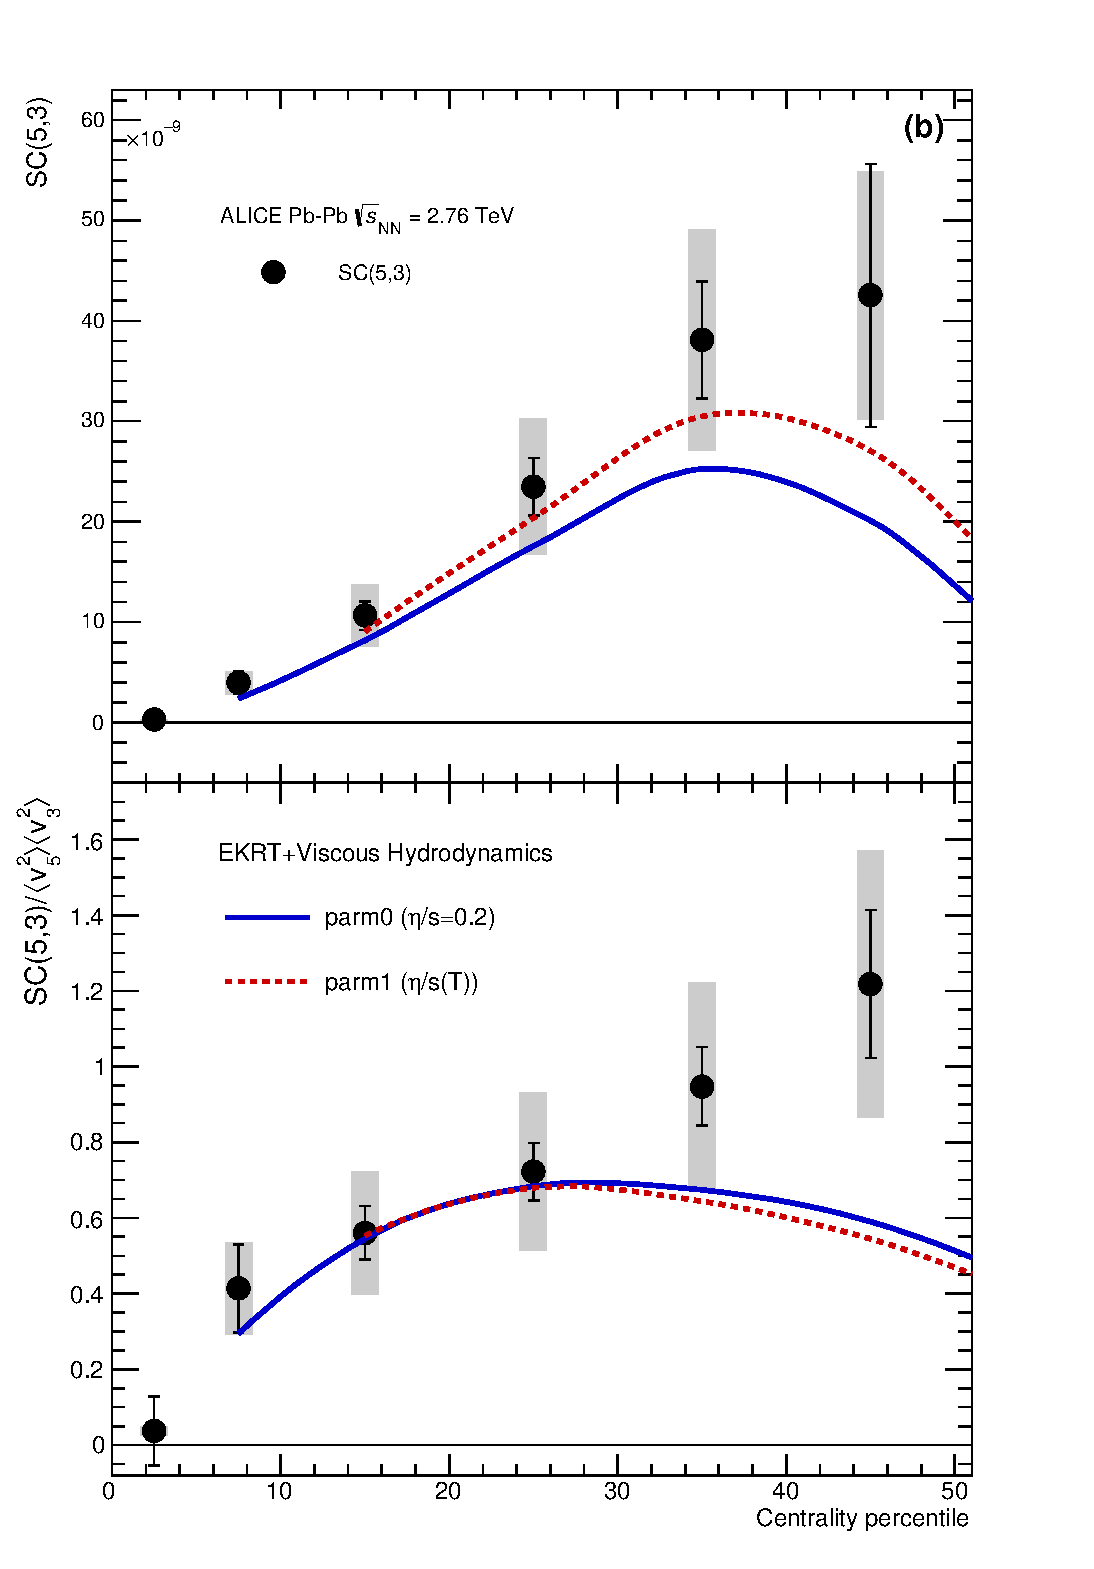
\includegraphics{figs/fig3_QConly_ModelComparison_SC53_EKRT.eps}}
                       \resizebox{0.32\textwidth}{!}{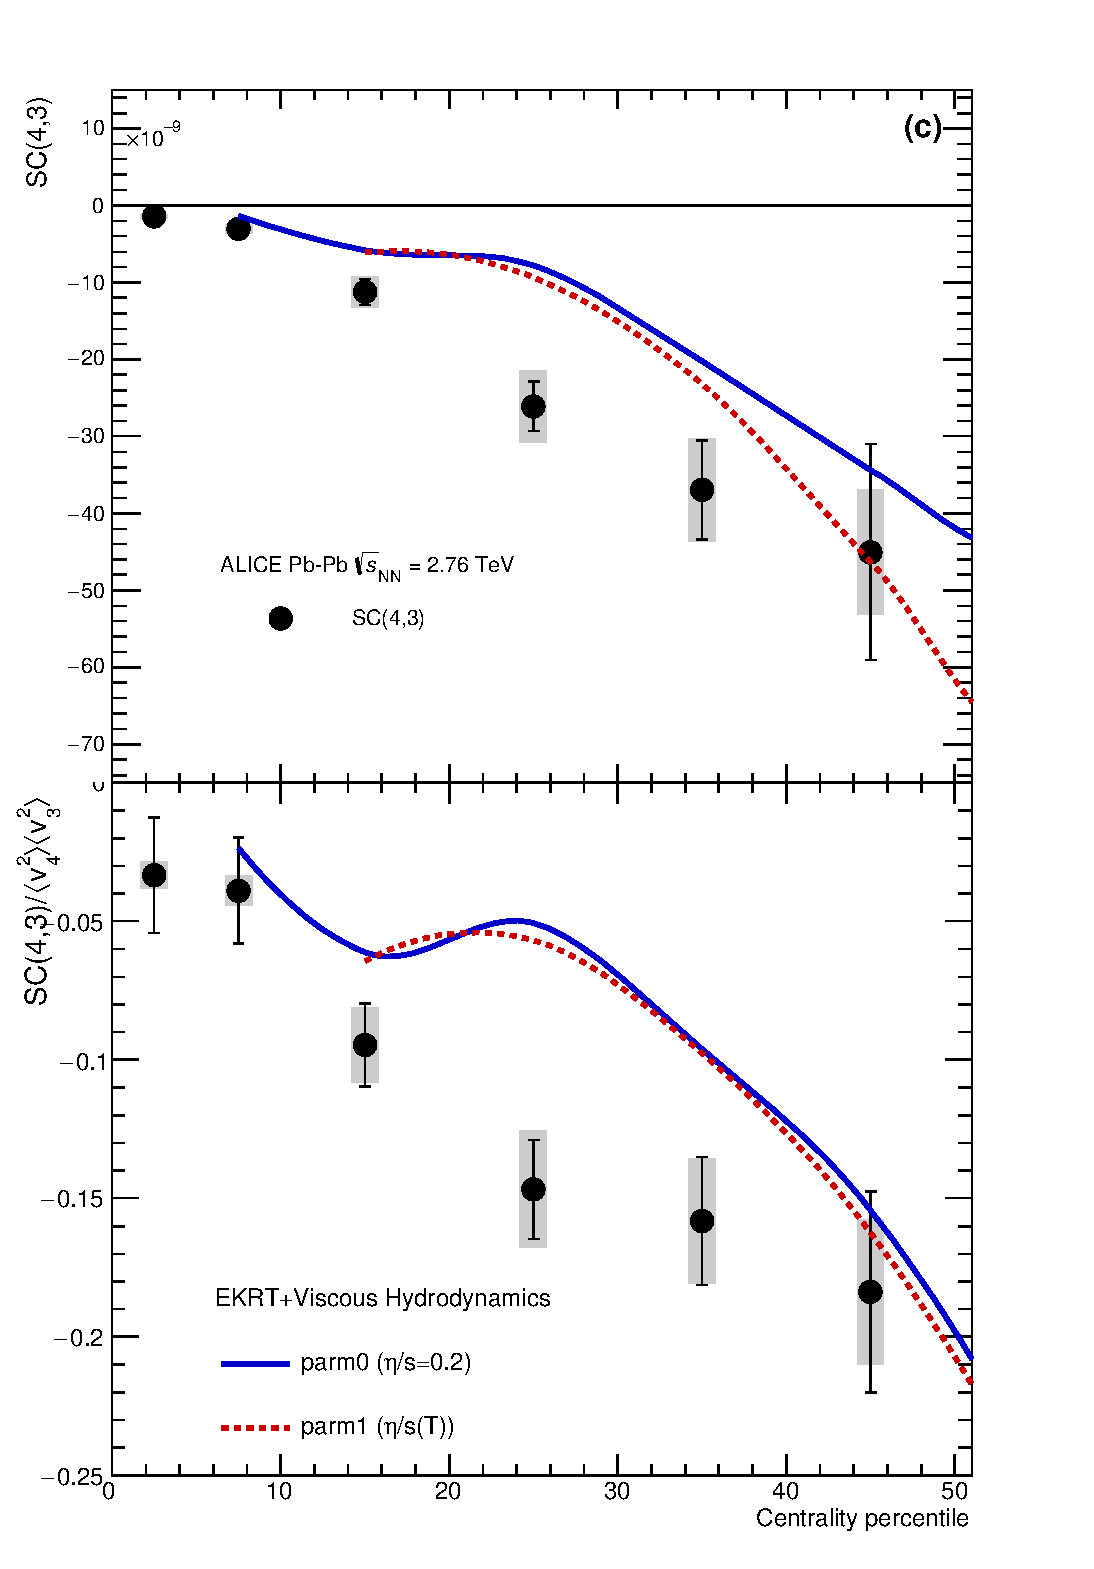
\includegraphics{figs/fig3_QConly_ModelComparison_SC43_EKRT.eps}}
              \end{center}
        \caption{Measurements of  SC(5,2) (a), SC(5,3) (b) and SC(4,3) (c) in $\PbPb$ collisions at $\snn=2.76$~TeV are compared to the event-by-event EKRT+viscous hydrodynamic calculations~\cite{Niemi:2015qia}. The lines are hydrodynamic predictions with two different $\eta/s(T)$ parameterizations, labeled in the same way as in ~\cite{Niemi:2015qia}. Upper (lower) panels show SC$(m,n)$ (NSC$(m,n)$).}        
        \label{fig:Figure_5}
\end{figure*}

The higher order harmonic correlations are compared to VISH2+1 calculations~\cite{Zhu:2016puf}, shown in Fig.~\ref{fig:Figure_6}. 
All the models with large $\eta/s$ ($\eta/s=0.2$ for MC-KLN and MC-Glauber, and $\eta/s=0.16$ for AMPT initial conditions) regardless of the initial conditions fail to capture the centrality dependence of SC(5,2), SC(5,2) and SC(5,3), with larger disagreements than observed for the lower order harmonic correlations.
Among the models with small $\eta/s$ ($\eta/s=0.08$), the one with the AMPT initial conditions describes the data much better than the ones with other initial conditions. 
A clear separation between different initial conditions is observed for these higher order harmonic correlations compared to the lower order harmonic correlations.
NSC(5,2) and SC(5,3) are quite sensitive to both the initial conditions and the $\eta/s$ parameterizations.
Similar to the hydrodynamic calculations mentioned above~\cite{Niemi:2015qia}, the sign of NSC(4,3) in these models is opposite to its sign in the data in 0--10\% central collisions. NSC(4,3) shows sensitivity to both initial conditions and $\eta/s$ parameterizations.
% while NSC(3,2) does not show sensitivity to initial conditions nor to different $\eta/s$ parameterizations.
The SC(4,3) results are clearly favored by smaller $\eta/s$ values but NSC(4,3) cannot be described by these models quantitively.
     
\begin{figure*}[!]
	\begin{center}
        	\resizebox{0.32\columnwidth}{!}{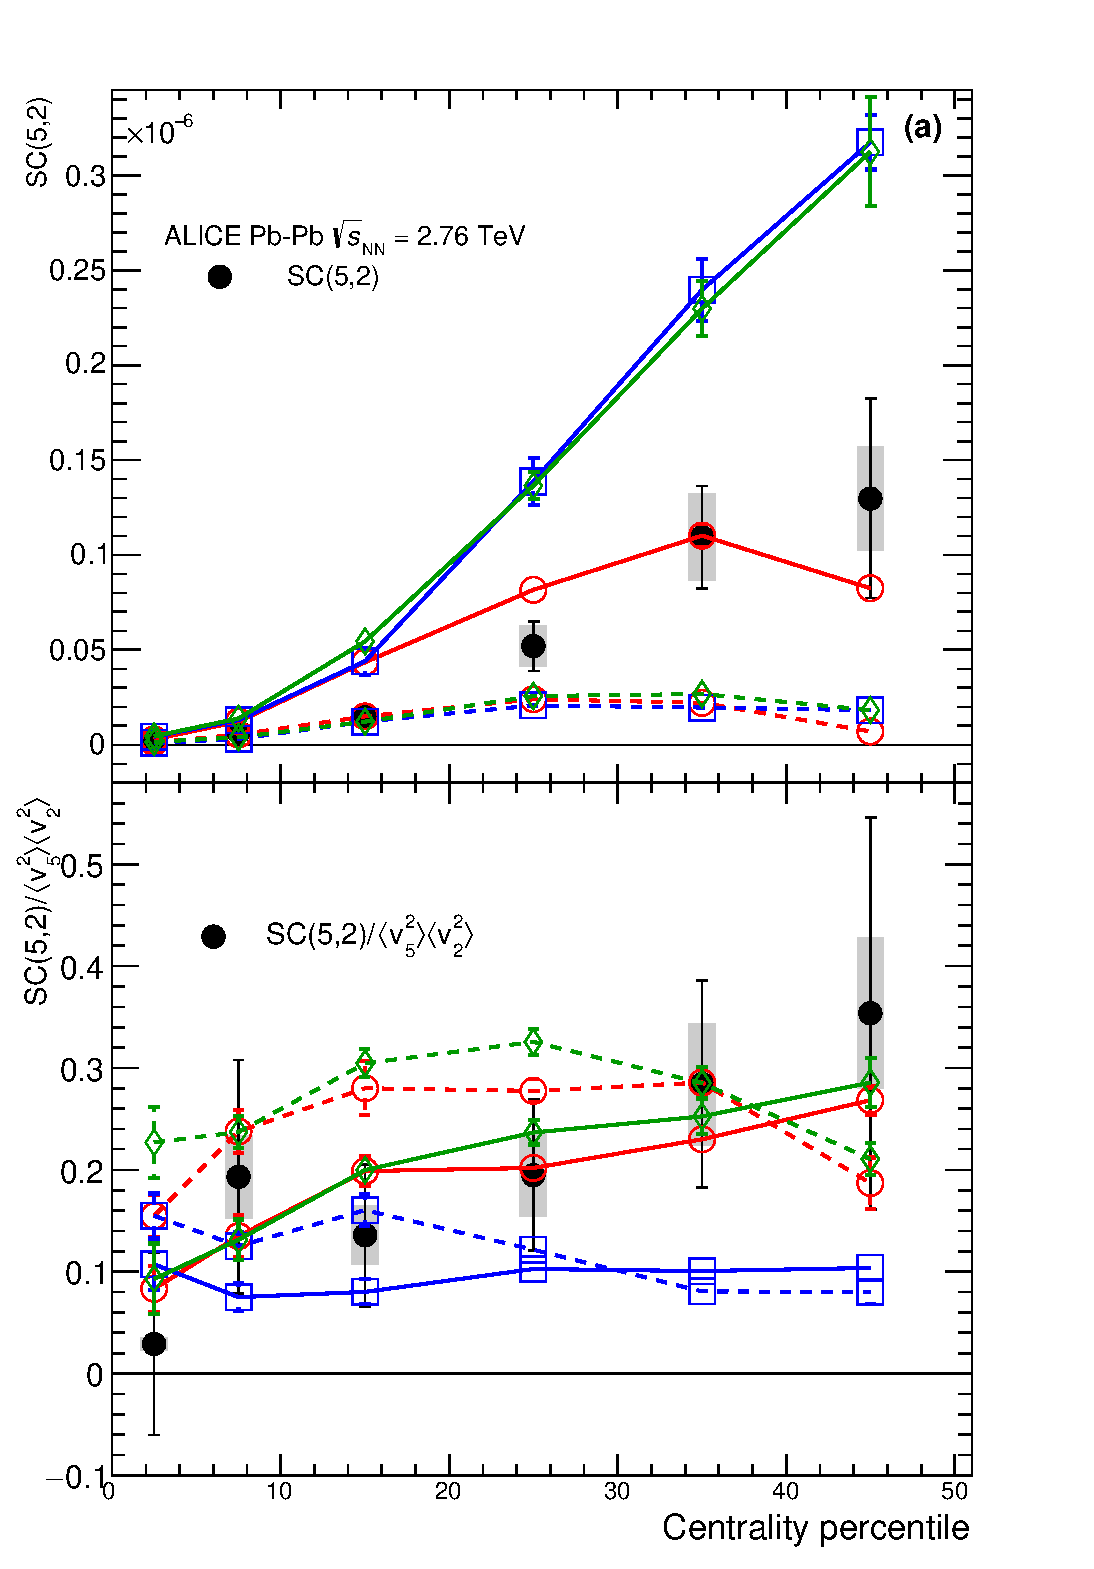
\includegraphics{figs/fig3_QConly_ModelComparison_SC52_vish.eps}}
        	\resizebox{0.32\columnwidth}{!}{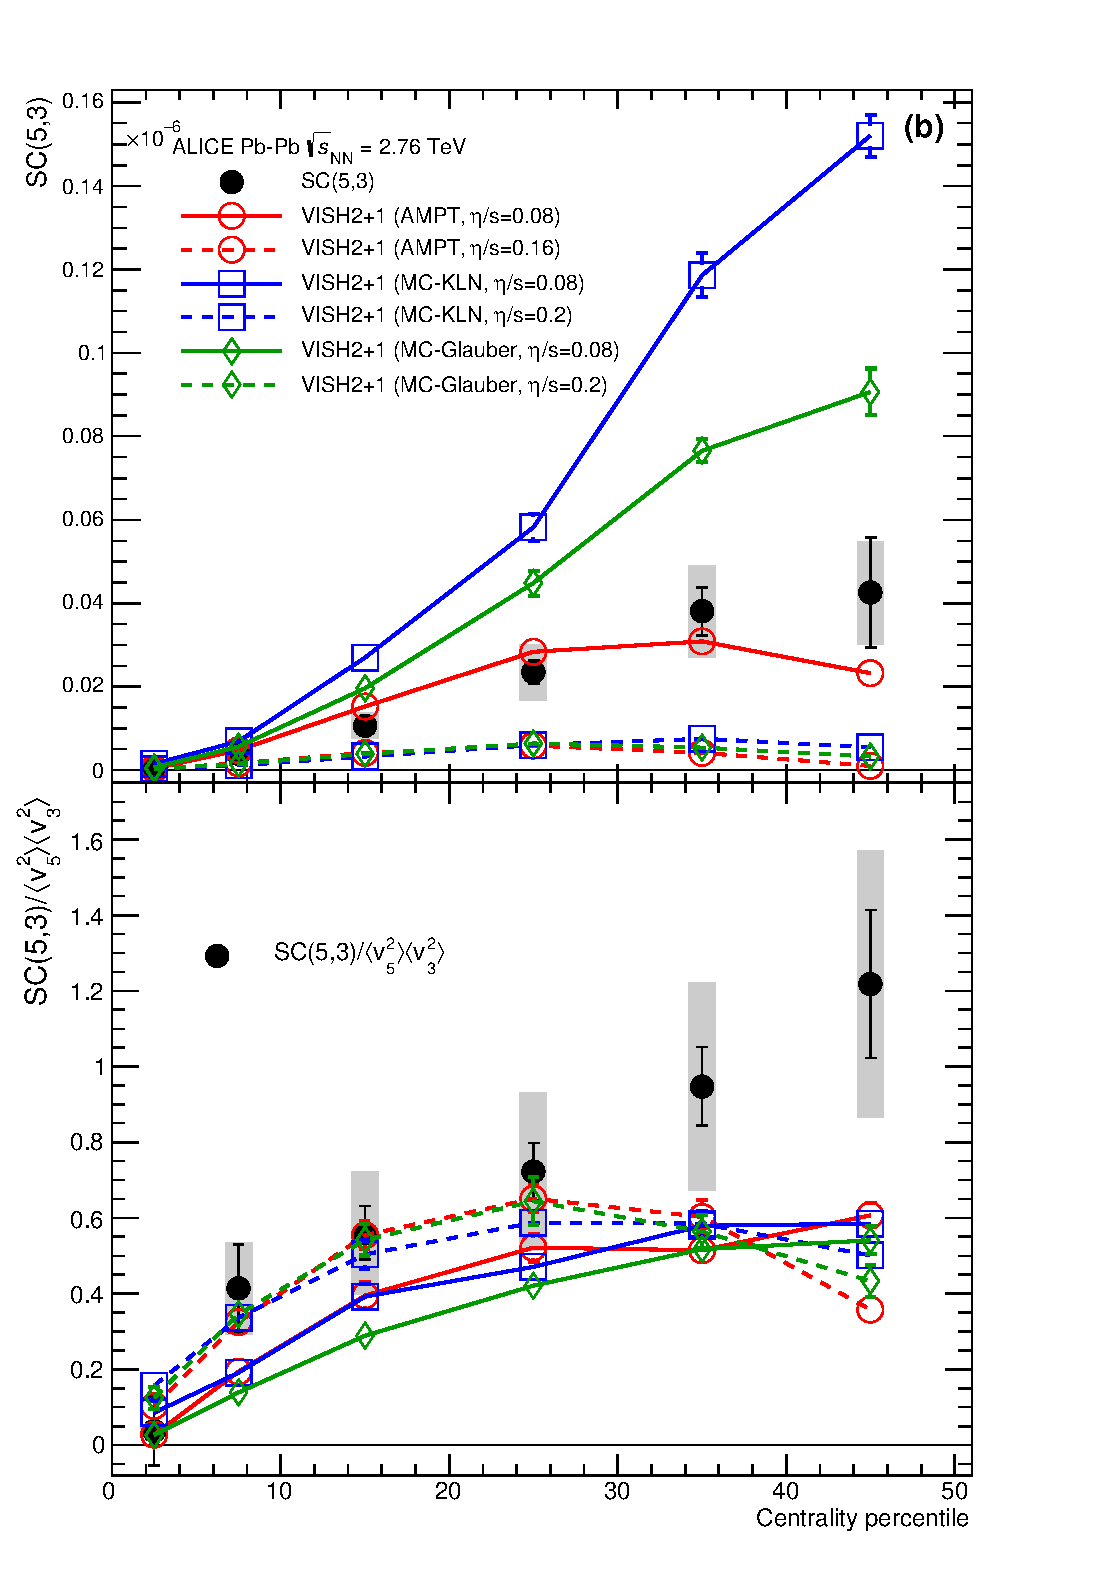
\includegraphics{figs/fig3_QConly_ModelComparison_SC53_vish.eps}}
        	\resizebox{0.32\columnwidth}{!}{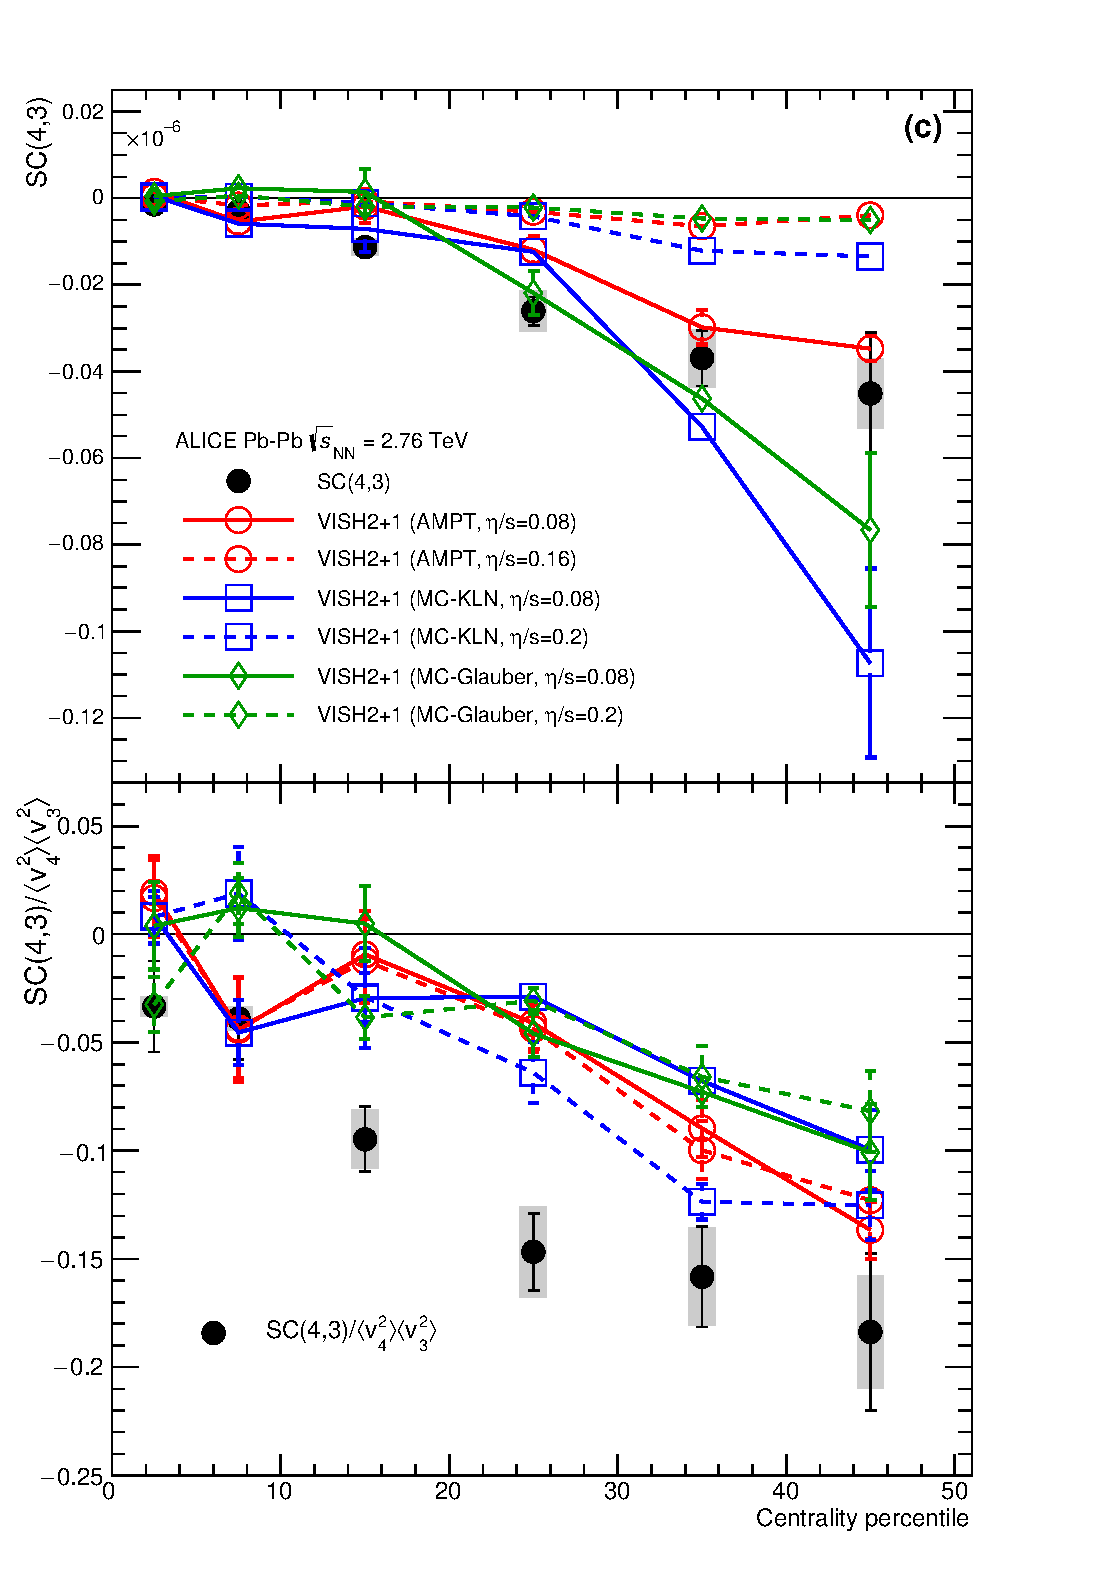
\includegraphics{figs/fig3_QConly_ModelComparison_SC43_vish.eps}}
        \caption{Results of  SC(5,2), SC(5,3) and SC(4,3) in $\PbPb$ collisions at $\snn=2.76$~TeV are compared to various VISH2+1 calculations~\cite{Zhu:2016puf}. Three initial conditions from AMPT, MC-KLN and MC-Glauber are drawn as different colors and markers. The $\eta/s$ parameters are shown as different line styles, the small shear viscosity ($\eta/s=0.08$) are shown as solid lines, and large shear viscosities ($\eta/s=0.2$ for MC-KLN and MC-Glauber, 0.16 for AMPT) are drawn as dashed lines. Upper (lower) panels show SC$(m,n)$ (NSC$(m,n)$).}
        \label{fig:Figure_6}
        \end{center}   
 \end{figure*}
 
 \begin{figure*}[!]
	\begin{center}
        	\resizebox{0.32\columnwidth}{!}{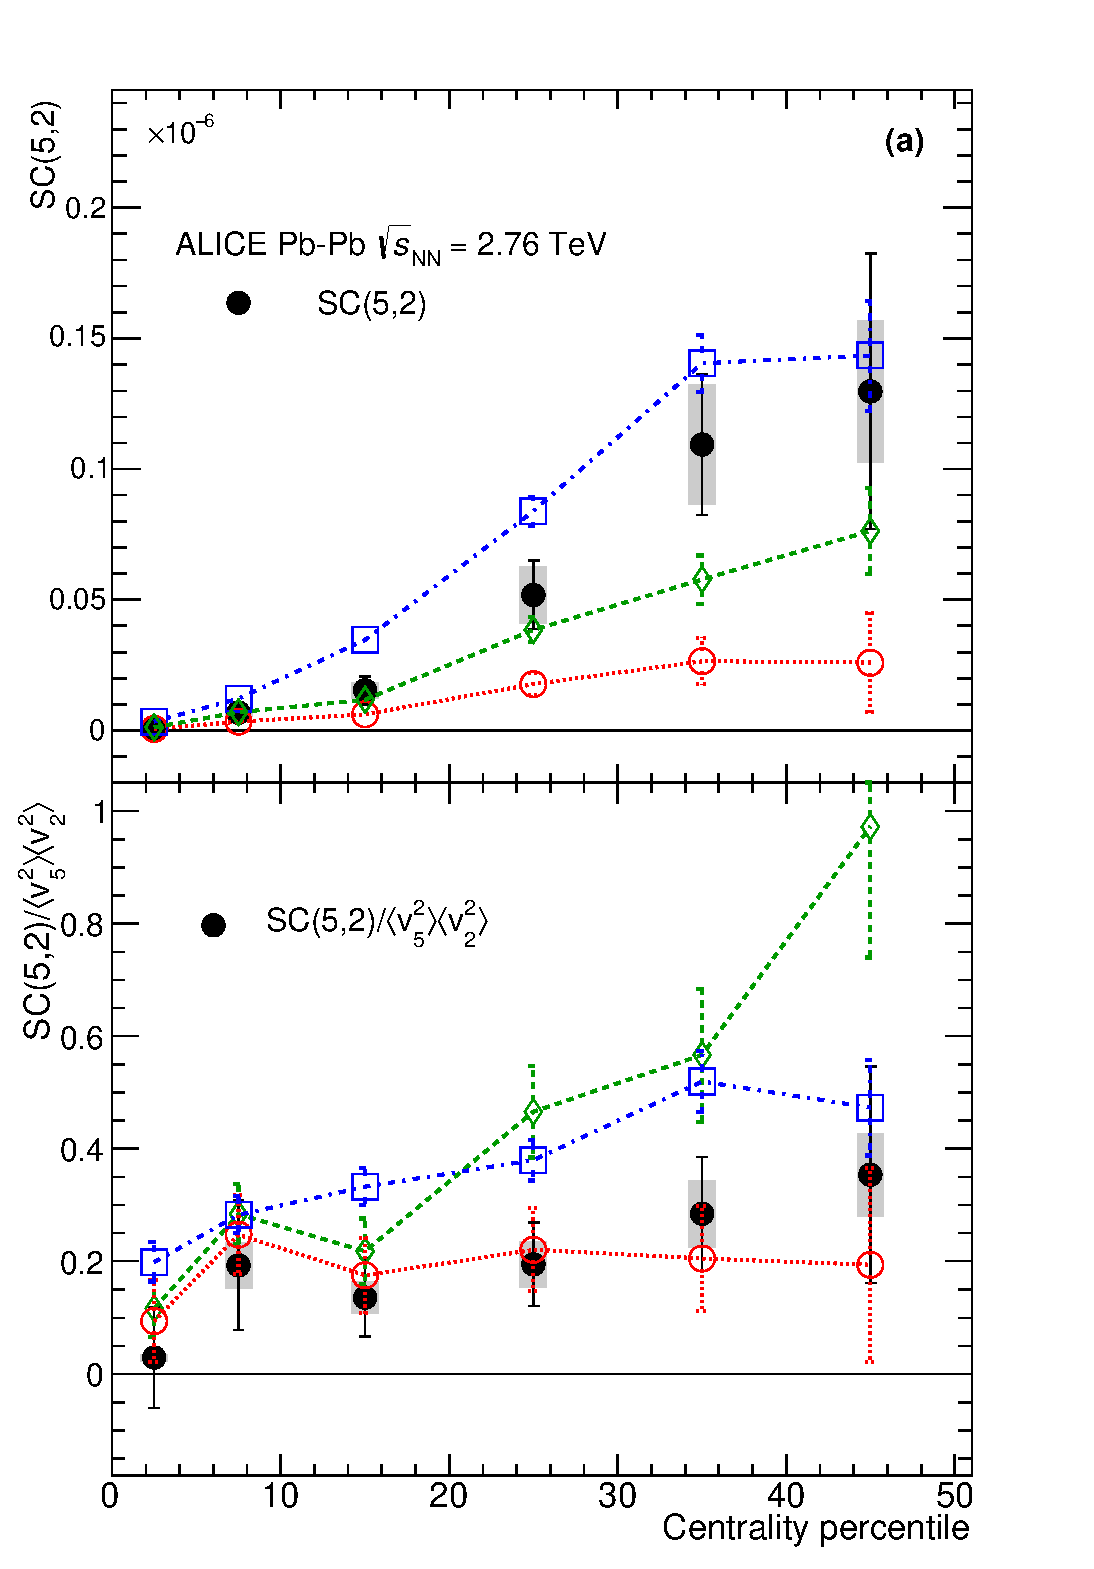
\includegraphics{figs/fig3_QConly_ModelComparison_SC52_ampt.eps}}
        	\resizebox{0.32\columnwidth}{!}{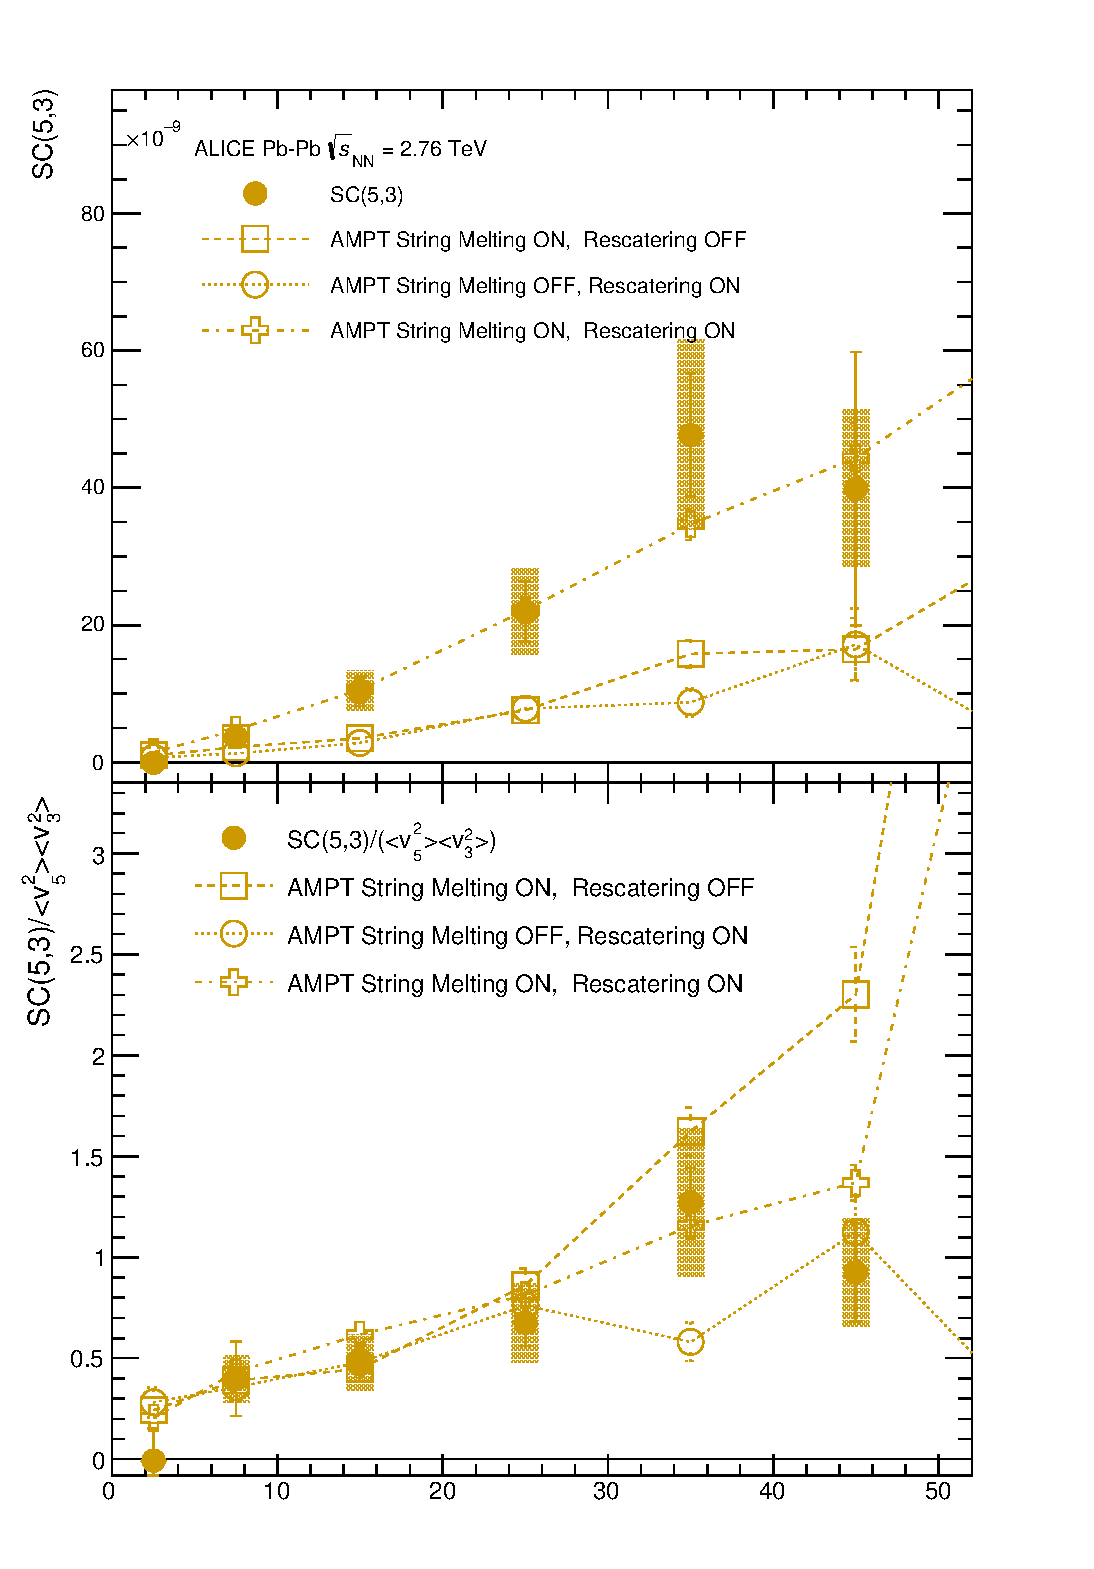
\includegraphics{figs/fig3_QConly_ModelComparison_SC53_ampt.eps}}
        	\resizebox{0.32\columnwidth}{!}{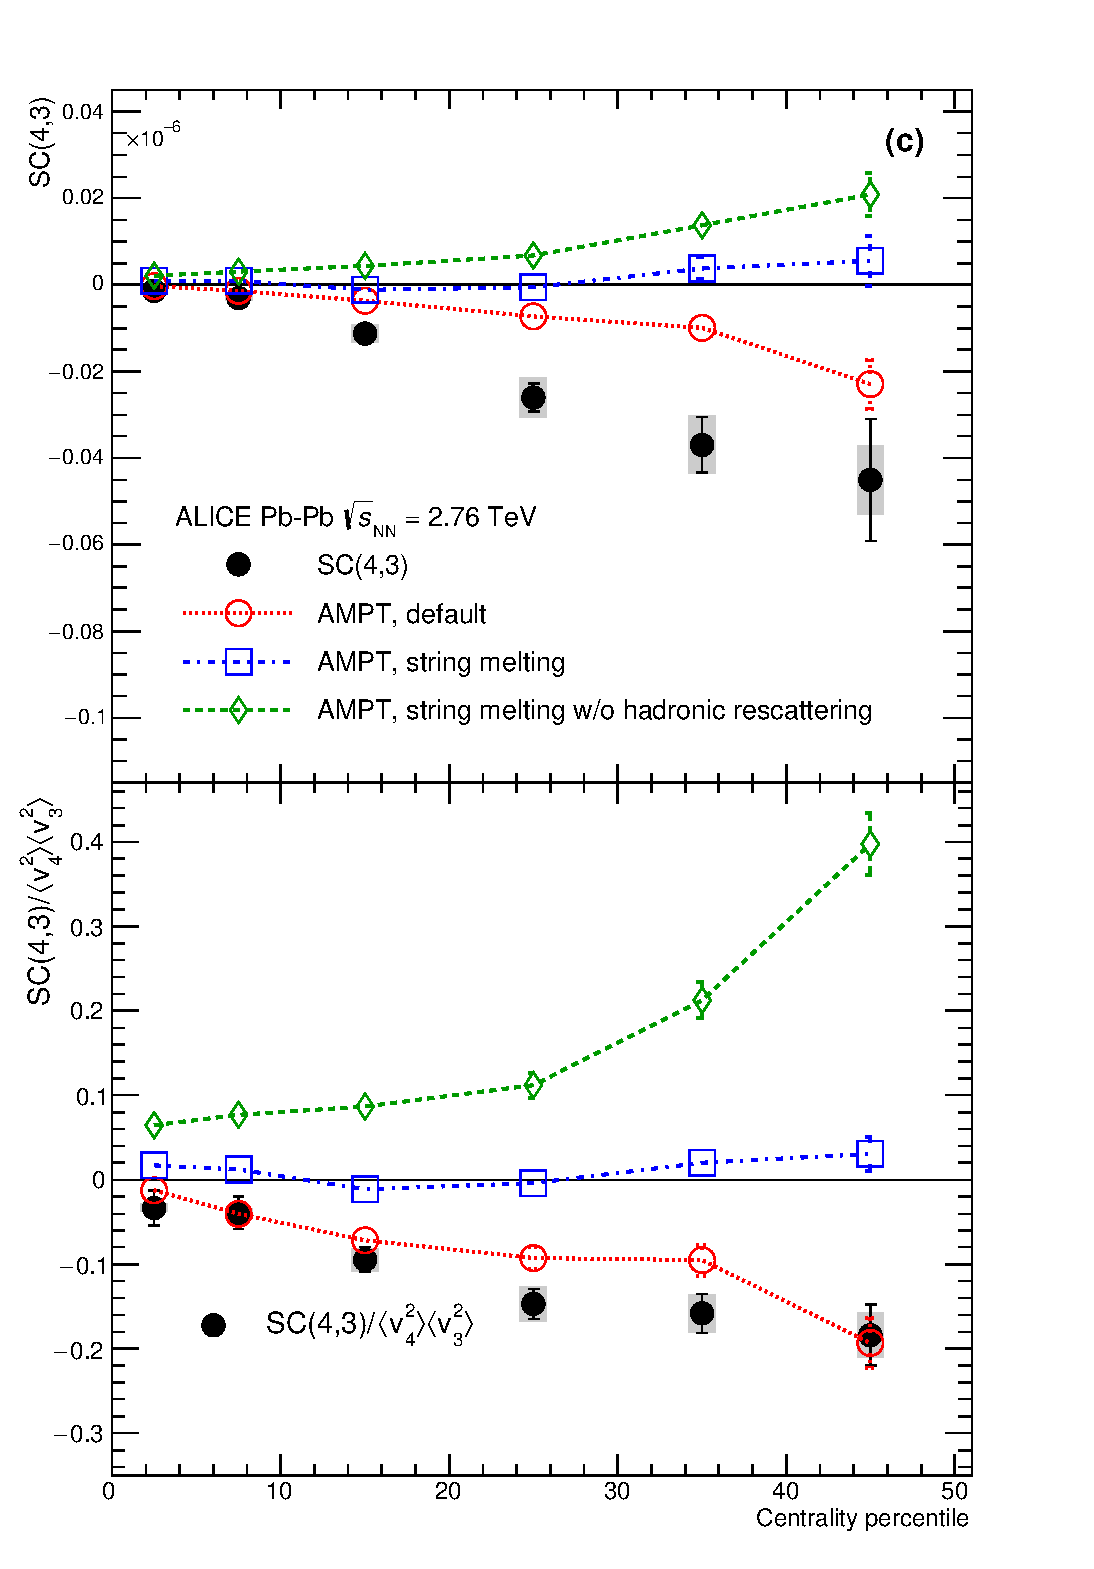
\includegraphics{figs/fig3_QConly_ModelComparison_SC43_ampt.eps}}
        \caption{Results of  SC(5,2), SC(5,3) and SC(4,3) in $\PbPb$ collisions at $\snn=2.76$~TeV are compared to various AMPT models. Upper (lower) panels show SC$(m,n)$ (NSC$(m,n)$).}
        \label{fig:Figure_7}
        \end{center}   
 \end{figure*}
 
The results from AMPT simulations are compared to the data in Fig.~\ref{fig:Figure_7}.
The string melting AMPT model describes SC(5,3) and NSC(5,3) well. However, the same setting overestimates SC(5,2) and NSC(5,2). 
The default AMPT model can describe NSC(5,3) and NSC(5,2) fairly well as in the case of the lower harmonics seen in Fig.~\ref{fig:Figure_4}.
% interesting AMPT String Melting OFF, Rescattering ON < AMPT String Melting ON, Rescattering OFF
In the case of SC(4,3), neither of the settings can describe the data but the default AMPT model comes the closest to the data. 
The string melting AMPT model fails to describe SC(4,3) and NSC(4,3).
In summary, the default AMPT model describes well the normalized symmetric cumulants (NSC$(m,n)$) from lower to higher order harmonic correlations while the string melting AMPT model overestimates NSC(5,2) and predicts a very weak correlation in NSC(4,3). 

%It should be noted that the better agreement for SC$(m,n)$ should not be overemphasized since there are discrepancies in the individual $v_n$ between AMPT and data as it was demonstrated for SC(3,2).
%Hence the simultaneous description of SC$(m,n)$ and NSC$(m,n)$ should give better constrains to the parameters in AMPT.
%Can we conclude that the hadronic rescattering only can reproduce the correlation strength well ?
%Considering the underestimated $NSC(4,3)$ in VISH2+1 calculation can be compensated by hadronic rescattering a.l.a ...... ?

As discussed in Sec.~\ref{sec:results}, a hierarchy NSC(5,3) $>$ NSC(4,2) $>$ NSC(5,2) holds for centrality ranges $>20\%$ within the errors and NSC(5,2) is smaller than NSC(5,3) while SC(5,2) is larger that SC(5,3).
Except for the 0--10\% centrality range, we found that the same hierarchy also holds in the hydrodynamic calculations and the AMPT models explored in this article.
The observed reversal of the hierarchy SC(5,2) $>$ SC(5,3), can be explained by the magnitudes of the individual flow harmonics ($v_2$ $>$ $v_3$). 
The opposite trend is observed for the normalized SC (NSC(5,3) $>$ NSC(5,2)). This can be attributed to the fact that flow fluctuations are stronger for $v_3$ than $v_2$~\cite{Aad:2013xma}. This was claimed in Ref.~\cite{Zhu:2016puf} and also seen in Ref.~\cite{Bhalerao:2014xra} based on an AMPT model. 
NSC($m$,$n$) correlators increase with larger $\eta/s$ in hydrodynamic calculations in the 0-30\% centrality range in the same way as the event plane correlations~\cite{Bhalerao:2013ina,Teaney:2013dta}. In semi-peripheral collisions ($>$40\%), the opposite trend is observed.


We list here the important findings from the model comparisons:
\begin{enumerate}[(i)]
	\item All the VISH2+1 model calculations with large $\eta/s$ fail to capture the centrality dependence of the correlations regardless of the initial conditions.
	\item Among the VISH2+1 model calculations with small $\eta/s$ ($\eta/s=0.08$), the one with the AMPT initial conditions describes the data qualitatively but it cannot describe the data quantitively for most of the centrality ranges.
	\item The NSC(3,2) observable is sensitive mainly to the initial conditions, while the other observables are sensitive to both the initial conditions and the temperature dependence of $\eta/s$.
	\item The correlation strength between $v_3$ and $v_2$ and between $v_4$ and $v_3$ (NSC(3,2) and NSC(4,3)) is significantly underestimated in hydrodynamic model calculations.
	\item The sign of NSC(3,2) in 0--10\% central collisions was found to be different in the data and the hydrodynamic model calculations while the default AMPT model can reproduce the sign.
	\item The default AMPT model can describe the normalized symmetric cumulants (NSC($m$,$n$)) quantitively for most centralities while the string melting AMPT model fails to describe them.
	%\item The hadronic rescattering in AMPT model makes the correlation strength (NSC) larger.
	\item A hierarchy NSC(5,3) $>$ NSC(4,2) $>$ NSC(5,2) holds for centrality ranges $>20\%$ within the errors. This hierarchy is reproduced well both by hydrodynamic and AMPT model calculations.

\end{enumerate}


\subsection{Transverse Momentum Dependence of Correlations between $v_2$, $v_3$ and $v_4$}
\label{sec:ptdepsc}

It can be seen in Fig.~\ref{fig:Figure_2} that for NSC(3,2) there is no $p_{\rm T, min}$ dependence in the centrality range $<$30\%, and a moderate decreasing trend with increasing $p_{\rm T, min}$ is observed in the $>$30\% centrality range.
NSC(4,2) shows a moderate decreasing trend as $p_{\rm T, min}$ or centrality increases. 
In order to see the trend more clearly, we show NSC($m$,$n$) results as a function of minimum $p_{\rm T}$ cut in Figs.~\ref{fig:Figure_8} and \ref{fig:Figure_9}.

\begin{figure}[p]
             \begin{center}
              \resizebox{0.95\textwidth}{!}{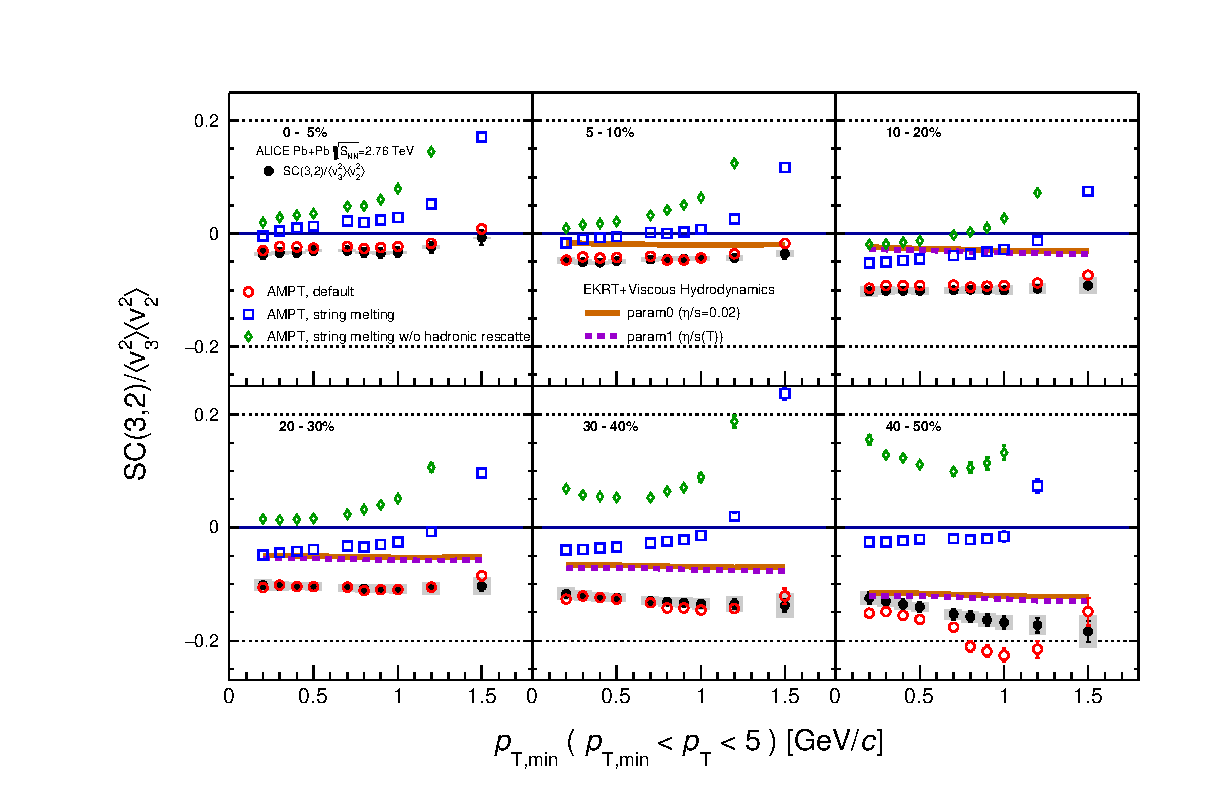
\includegraphics{figs/fig5_QConly_xminpt_nSC32_EKRT.eps}}
              \end{center}
             \caption{NSC(3,2) as a function of the minimum $p_{\rm T}$ cut in $\PbPb$ collisions at $\snn=2.76$~TeV is compared to various AMPT configurations and event-by-event EKRT+viscous hydrodynamic calculations~\cite{Niemi:2015qia}.}
             \label{fig:Figure_8}
\end{figure}

\begin{figure}[p]
             \begin{center}
              \resizebox{0.95\textwidth}{!}{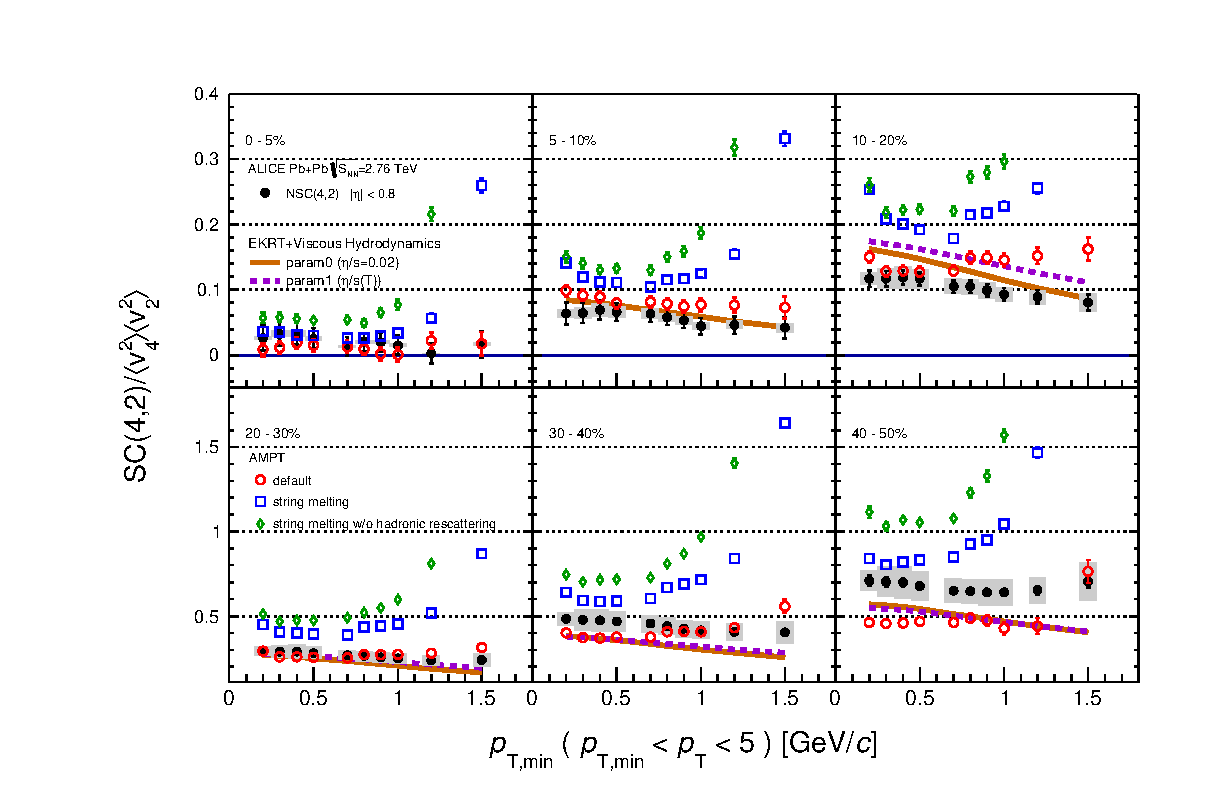
\includegraphics{figs/fig5_QConly_xminpt_nSC42_EKRT.eps}}
              \end{center}
             \caption{NSC(4,2) as a function of the minimum $p_{\rm T}$ cut in $\PbPb$ collisions at $\snn=2.76$~TeV is compared to various AMPT configurations and event-by-event EKRT+viscous hydrodynamic calculations~\cite{Niemi:2015qia}.}
             \label{fig:Figure_9}
\end{figure}

NSC(3,2) and NSC(4,2) as a function of $p_{\rm T, min}$ are compared to the {AMPT} simulations in Fig.~\ref{fig:Figure_8} and Fig.~\ref{fig:Figure_9}, respectively.
The observed $p_{\rm T}$ dependence for NSC(3,2) and NSC(4,2) in mid-central collisions is also seen in AMPT simulations for higher minimum $p_{\rm T}$ cuts.
With the exception of the default configuration, the other AMPT settings predict a very strong $p_{\rm T}$ dependence above 1~GeV/$c$ and cannot describe the magnitudes of both NSC(3,2) and NSC(4,2) simultaneously.
In the case of NSC(3,2), the default AMPT model describes the magnitude and $p_{\rm T}$ dependence well in all collision centralities except for $40-50\%$ where the model underestimates the data and shows a stronger $p_{\rm T}$ dependence than the data.
As for  NSC(4,2), the same model which describes NSC(3,2) can also reproduce the data well except for the $10-20\%$ and $40-50\%$ centralities where some deviations are observed.
When the string melting AMPT model is compared to the same model with the hadronic rescattering off, it is observed that the very strong $p_{\rm T}$ dependence as well as the correlation strength are weakened by the hadronic rescattering.
This might imply that hadronic interactions are the source of this observed $p_{\rm T}$ dependence even though the relative contributions from the partonic and hadronic stages in the final state particle distributions should be studied further.

The event-by-event EKRT+viscous hydrodynamic calculations are compared to the data in Fig.~\ref{fig:Figure_8}.
In the case of NSC(3,2), the hydrodynamic calculations underestimate the data as discussed in Sec~\ref{sec:theory_loworder} and show very weak $p_{\rm T}$ dependence for all centralities.
The $p_{\rm T}$ dependence of NSC(3,2) is well described by the model calculations in all collision centralities except for 40--50\% where the data shows stronger $p_{\rm T}$ dependence than the models. The difference between the model calculations with the two different parameterizations of $\eta/s(T)$ is very small. 
As for NSC(4,2), the model calculations overestimate the result in the 5--20\% centralities and underestimate it in the centrality range $>$~20\%. However, the $p_{\rm T}$ dependence is well described by the model calculations in all centrality range. 
While the difference of the model results for the two parameterizations in most centralities is rather small, a clear separation between the two are observed in the 10--20\% centrality range where both the magnitude and $p_{\rm T}$ dependence are different.

This observed moderate $p_{\rm T}$ dependence in mid-central collisions both for NSC(3,2) and NSC(4,2) might be an indication of possible viscous corrections to the equilibrium distribution at hadronic freeze-out as predicted in ~\cite{Niemi:2012aj}.
The comparisons to hydrodynamic models can further help to understand the viscous corrections to the momentum distributions at hadronic freeze-out~\cite{Dusling:2009df,Luzum:2010ad,Teaney:2012ke,Molnar:2014fva,Niemi:2015qia}.
%\noindent\textbf{\textcolor{blue}{[Waiting for $\eta/s(T)$ hydro calculations from Harri Niemi et. al~\cite{} and VISH2+1 calculations~\cite{Zhu:2016puf}]}}


 
\section{Summary}
\label{sec:summary}
In this article, we report the centrality dependence of correlations between the higher order harmonics ($v_4$, $v_5$) and the lower order harmonics ($v_2$, $v_3$) as well as the transverse momentum dependence of the correlations between $v_3$ and $v_2$ and between $v_4$ and $v_2$.
The results are obtained with Symmetric 2-harmonic 4-particle Cumulants (SC). It was demonstrated earlier in \cite{ALICE:2016kpq} that this method is insensitive to non-flow effects and independent of symmetry plane correlations.
We have found that fluctuations of SC(3,2) and SC(4,3) are anti-correlated in all centralities while fluctuations of SC(4,2), SC(5,2) and SC(5,3) are correlated for all centralities. 
These measurements were compared to various hydrodynamic model calculations with different initial conditions as well as different parameterizations of the temperature dependence of $\eta/s$.
It is found that the different order harmonic correlations have different sensitivities to the initial conditions and the system properties. Therefore they have discriminating power in separating the effects of $\eta/s$  from the initial conditions on the final state particle anisotropies.
The sign of SC(3,2) in 0--10\% central collisions was found to be different between the data and hydrodynamic model calculations.
In the most central collisions the anisotropies originate mainly from fluctuations, where the initial ellipsoidal geometry which dominates in mid-central collisions plays little role. This observation might help to understand the details of the fluctuations in the initial stage. 
The comparisons to VISH2+1 calculations show that all the models with large $\eta/s$, regardless of the initial conditions, fail to capture the centrality dependence of higher order correlations. 
Based on the tested model parameters, the data favors small $\eta/s$ and the AMPT initial conditions. A quite clear separation of the correlation strength for different initial conditions is observed for these higher order harmonic correlations compared to the lower order harmonic correlations.
The default configuration of the AMPT model describes well the normalized symmetric cumulants (NSC($m$,$n$)) for most centralities and for most combinations of harmonics which were considered. %Together with the measurements of individual harmonics these results provide further constraints on the system properties and help discriminate between theoretical models.
Finally, we have found that $v_3$ and $v_2$ as well as $v_4$ and $v_2$ correlations have moderate $p_{\rm T}$ dependence in mid-central collisions. This might be an indication of possible viscous corrections to the equilibrium distribution at hadronic freeze-out.
Together with the measurements of individual harmonics these results presented in this article can be used to further optimize model parameters and put better constraints on the initial conditions and the transport properties of nuclear matter in ultra-relativistic heavy-ion collisions.

%\section{Outlooks}
%\label{sec:outlook}
%Interpretation of flow results obtained with multiparticle correlation techniques in small colliding systems, like pp and p--Pb at LHC, remains a challenge. The underlying difficulty stems from the fact that when anisotropic flow harmonic $v_n$ is estimated with $k$-particle correlator, the statistical spread of that estimate scales to leading order as $\sigma_{v_{n}}\sim\frac{1}{\sqrt{N}}\frac{1}{M^{k/2}}\frac{1}{v_{n}^{k-1}}$, where $M$ is the number of particles in an event (multiplicity) and $N$ is total number of events. This generic scaling ensures that multiparticle correlations are precision method only in heavy-ion collisions, characterized both with large values of multiplicity and flow. To leading order the measurements in small systems~\cite{Aad:2013fja,Abelev:2014mda,Khachatryan:2015waa,Adamczyk:2015xjc,Adare:2015ctn} and the measurements in heavy-ion collisions resemble the same features, which can be attributed to collective anisotropic flow in both cases. However, such interpretation is challenged by the outcome of recent Monte Carlo study~\cite{Loizides:2016tew} for $e^+e^-$ systems in which collective effects are not expected. Nonetheless, in this study to leading order multiparticle correlations exhibit yet again the similar universal trends first seen in heavy-ion collisions, both for elliptic and triangular flow. Therefore, it seems unlikely that the analysis of individual flow harmonics with multiparticle techniques will answer whether collective effects can develop and QGP be formed in small systems.
%%Instead observables like SC may shed light on multiparticle correlation measurements in pp and p--Pb. 
%%%%instead new observables, like SC, might provide the final answer due to their better sensitivity~\cite{Niemi:2012aj,ALICE:2016kpq}.

